
\section{\label{sec:intro_fe}Introduction}

The next generation of nuclear medicine would appear to be based upon the production of novel, emerging radionuclides \cite{Qaim201731}. 
The targeted and personalized nature of therapy and imaging applications using these novel radionuclides  makes possible an improvement in clinical practice, offering many patients the possibility for better survival rates and quality lives \cite{Mulford2005,Muller2014}.
While the chemical and radioactive decay properties of many of these radionuclides are well-established, their broad-scale  clinical applications are reliant upon well-characterized nuclear data to facilitate large-scale   production. 
% The future of nuclear medicine would appear to be the paradigm of personalized medicine --- targeted radionuclide therapy to spare healthy tissue \cite{Mulford2005,Qaim201731}, and theranostic medicine, which pairs an imaging isotope with a therapeutic isotope (frequently, of the same element), to provide simultaneous, real-time dose delivery and verification, leading to drastic reductions in prescribed patient dose \cite{Muller2014,Bentzen2005,Srivastava2012}. 
% Other variants of theranostic medicine exist, including pre-imaging for treatment planning, or delivery of a single compound with different radioelements for imaging/therapy where the inter-element biodistribution has been validated.  
% Change up the next sentance a bit
% Novel applications are being explored for several radionuclides whose production methodologies are not established, but their production requires accurate, high-fidelity cross section data.
% \cite{Qaim201731}. 
% Many of these applications focus on theranostics, the use of chemically identical (or similar) imaging and therapeutic radiopharmaceuticals for treatment of disease. 
One particular group of  emerging radionuclides are the various positron-emitting isotopes of manganese, which have been identified as having potential for a range of diagnostic applications \cite{J.2013,Graves2015,Lewis2015,PhysRevC.96.014613,Wooten2017,Hernandez2017}.
In particular, a significant interest has been expressed in producing the emerging radionuclides \ce{^{51}Mn} for clinical use in metabolic PET studies, as well as  \ce{^{52g}Mn} for pre-clinical imaging of neural and immune processes via PET \cite{Graves2016}. 
As part of a larger campaign to address deficiencies in cross-cutting nuclear data needs, our group has performed a   measurement of the   nuclear excitation functions of the radionuclides \ce{^{51}Mn},   \ce{^{52m}Mn}, and \ce{^{52g}Mn}.
This was carried out in a  thin-foil stacked-target experiment, using proton irradiation of natural iron foils with titanium and copper monitor foils.
While recent work has been performed in the 40--100\,MeV energy region, this work seeks to complement these measurements and extend them down to reaction thresholds, to investigate the feasibility of production using the international network   of low-energy medical cyclotrons   \cite{Graves2016}. 


Manganese radionuclides are desirable for radiopharmaceutical applications, as manganese is a chemically versatile element, biologically relevant, and essential in trace quantities. 
Manganese possesses well-established biochemistry, and has been proven to be chelated well by DOTA for tracking monoclonal antibodies, with high biostability at neutral pH \cite{Graves2015}.
\ce{^{52}Mn} ($t_{1/2}$ = 5.591$\pm$0.003\,d, $I_{\beta^+}$ = 29.4\%, $E_{\beta\text{, avg}}$ = 0.242\,MeV) has been shown to be useful for immunoPET applications, with its rapid blood clearance offering the possibility for imaging within minutes of injection \cite{Dong2015}.
Its lifetime allows for immunoPET imaging up to 2--3 weeks after administration, giving \ce{^{52}Mn} a longer duration for useful imaging  than the more established immunoPET agents \ce{^{89}Zr} or   \ce{^{64}Cu} \cite{Graves2015}. 
\ce{^{52}Mn}  has high uptake in the heart, liver, kidneys, and pancreas, making it a useful diagnostic agent for pancreatic $\beta$-cell, insulinoma, and porphysome imaging. 
However, its  long lifetime and unfavorable decay gamma-rays (notably, its  744.233\,keV [$I_\gamma = 90.0\,\pm\,1.2\%$], 935.544\,keV [$I_\gamma = 94.5\,\pm\,1.3\%$], and 1434.092\,keV [$I_\gamma = 100.0 \pm 1.4\%$] lines) make it undesirable for clinical applications, but easily shipped worldwide and highly suitable for pre-clinical imaging \cite{Dong2015}.
The \ce{^{52m}Mn} isomer ($t_{1/2}$ = 21.1$\pm$0.2\,min, $I_{\beta^+}$ = 96.6\%, $E_{\beta\text{, avg}}$ = 1.172\,MeV) offers a much stronger positron emission branch than \ce{^{52g}Mn}, but its short lifetime makes production and handling difficult, and its  high-intensity gamma emission (1434.06\,keV [$I_\gamma = 98.2\,\pm\,0.5\%$]) contributes significantly to patient dose  \cite{Dong2015}.
Another emerging manganese radionuclide is \ce{^{51}Mn} ($t_{1/2}$ = 46.2$\pm$0.1\,min, $I_{\beta^+}$ = 97.09\%, $E_{\beta\text{, avg}}$ = 0.973\,MeV), whose short lifetime makes it clinically suited for rapid metabolic studies \cite{Wang2017}.
\ce{^{51}Mn} has a comparable positron branch and energy to \ce{^{52m}Mn}, more suitable for clinical use than the soft positron emissions of \ce{^{52g}Mn}. 
In addition, \ce{^{51}Mn} lacks any strong decay gamma-rays (its longer-lived daughter \ce{^{51}Cr} [$t_{1/2}$ = 27.704$\pm$0.003\,d] has only a single  320.0284\,keV [$I_\gamma = 9.910\,\pm\,0.010\%$] line), making it the best choice of these radionuclides for clinical imaging applications \cite{Wang2017}.








% While these efforts have been targeted towards the production cross section of the \ce{^{51,52g,52m}Mn} PET isotopes (as well as other emerging medical radionuclides produced in these irradiations), these measurements offer insight into the spin distribution of excited nuclear states, in the 5--55 MeV range.


% In addition to the interest in the production of\ce{^{51,52g,52m}Mn} for PET research

While these efforts have been motivated by the production cross section of the \ce{^{51,52g,52m}Mn} radionuclides for PET studies, this experiment offers an opportunity to study the distribution of angular momentum in compound nuclear and direct pre-equilibrium reactions via observation of the \ce{^{52m}Mn} ($t_{1/2}$ = 21.1$\pm$0.2\,min; J$^\pi=2+$) to \ce{^{52g}Mn} ($t_{1/2}$ = 5.591$\pm$0.003\,d; J$^\pi=6+$)   ratio \cite{Dong2015,Wang2017}.
Measurements of isomer-to-ground state ratios have been used for over 20\,years to probe the spin distribution of excited nuclear states in the A\,$\approx$\,190 region \cite{PhysRevC.73.034613,PhysRevC.45.1171}.
These measurements provide a range of cross section data invaluable to not only the medical isotope production community, but  also serve to measure the spin distribution in f$_{7/2}$ subshell nuclei via the observation of isomer-to-ground state ratios, and  as new data to improve the predictive capabilities of  reaction modeling codes. 
In addition, these experiments provide valuable insight into the challenges  involved in precision cross section data measurements. 



% A set of measured cross sections for the various natFe(p,x), natTi(p,x), and natCu(p,x) reactions between 5–55 MeV, as well as independent measurements of isomer branching ratios, are reported.
% Figure 3 shows the 52mMn(2+)/52gMn(6+) isomer-to-ground state branching ratio for the naFe(p,αn) reaction, calculated using TALYS-v1.8 over the 20 - 55 MeV range spanned by the foil stack. It is possible to use this measurement to infer the spin cut-off σ2, the width of the angular momentum distribution of the level density [6], [7]. The isomer-to-ground state ratio lends insight into equilibrium / pre-equilibrium nature of reactions in this energy region, useful when attempting to minimize dose from an unwanted isomer/ground state of a medical radionuclide.



% While this might seem obvious, the contributions to the slowing of the beam due to the adhesive has often been neglected in much work performed to date. While plays a limited role at high beam energies, it becomes increasingly important for proton energies below 25 MeV. 




% In addition to providing a potentially highly-valuable beam monitor, the Nb(p,x) reactions offer an opportunity to study the angular momentum deposition via pre-equilibrium reactions and the spin distribution in f$_{7/2}$ subshell nuclei via the observation of isomer-to-ground state ratios.  





% lee stuff:
% 
% In addition to the interest in the production of 51,52 Mn for PET research, this experiment offered
% an opportunity to study the distribution of angular momentum in compound nuclear and direct
% pre-equilibrium reactions via observation of the 52g Mn (t ½ =5.591±0.003 d; J π =6 + ) to 52m Mn
% (t ½ =21.1±0.2 m; J π =2 + ) ratio. These results indicated were presented at the University of Oslo in
% May 2017 5 and indicate that the constant
% temperature nuclear level density model
% which has had the greatest success at
% reproducing most low-energy nuclear
% reaction data fails to reproduce the
% deposition of angular momentum at both
% compound and pre-compound energies
% (see figure 3). This result will be
% discussed in greater detail in Mr. Andrew
% Voyles’ doctoral dissertation, which is
% expected to be completed by May 2018.
% 
% An important outcome from this work has an appreciation for the role played by the latex
% adhesive on the Kapton tape used to contain the individual stacked targets. While this might
% seem obvious, the contributions to the slowing of the beam due to the adhesive has been
% neglected in work performed at LANL-IPF to date. While this is expected to play a limited role
% at high beam energies, it becomes increasingly important for proton energies below 25 MeV.








% This sample document demonstrates proper use of REV\TeX~4.1 (and
% \LaTeXe) in mansucripts prepared for submission to APS
% journals. Further information can be found in the REV\TeX~4.1
% documentation included in the distribution or available at
% \url{http://authors.aps.org/revtex4/}.
% 
% When commands are referred to in this example file, they are always
% shown with their required arguments, using normal \TeX{} format. In
% this format, \verb+#1+, \verb+#2+, etc. stand for required
% author-supplied arguments to commands. For example, in
% \verb+\section{#1}+ the \verb+#1+ stands for the title text of the
% author's section heading, and in \verb+\title{#1}+ the \verb+#1+
% stands for the title text of the paper.
% 
% Line breaks in section headings at all levels can be introduced using
% \textbackslash\textbackslash. A blank input line tells \TeX\ that the
% paragraph has ended. Note that top-level section headings are
% automatically uppercased. If a specific letter or word should appear in
% lowercase instead, you must escape it using \verb+\lowercase{#1}+ as
% in the word ``via'' above.

\section{\label{sec:experimental_fe}Experimental Methods and Materials}


The work described herein follows the  methods utilized in our recent work and established by Graves \etal\ 
% for the measurement of cross sections in stacked target irradiations   
for monitor reaction characterization of beam energy and fluence in stacked target irradiations \cite{Voyles2018a,Graves2016}.
% 
% Make sure to add this back in for the journal article
% 
% 
% Preliminary analysis  was previously reported in the Master's thesis of one co-author, but the conclusive results of this work are described here  \cite{springer2017investigation}.

% \comment{Do we really need to cite Alex's thesis?}


\subsection{\label{sec:target_design_fe}Stacked-target design}

\comment{Update these energies, post-analysis}

A pair of target stacks were constructed for this work, due to the large energy range desired to be spanned.
One stack covers the \textred{55--20}\,MeV range and the other covers \textred{25--5}\,MeV, to minimize the systematic uncertainties associated with degradation of beam energy.
In addition, the complementary  energy  of the  stacks helps build confidence  through multiple overlapping measurements between 20--25\,MeV.  
% A stacked-target design was utilized for this work in order that the (p,x) cross sections for each reaction channel could be measured at multiple energy positions in a single irradiation \cite{Cumming1963}. 
% For targets, a
A series of nominal 25\,\mmicro m \ce{^{nat}Fe} foils (99.5\%\cmmnt{, \textred{lot \#T23A035}}), 25\,\mmicro m \ce{^{nat}Ti} foils (99.6\%\cmmnt{, \textred{lot \#M06C032}}), and 25\,\mmicro m \ce{^{nat}Cu} foils (99.95\%\cmmnt{, \textred{lot \#N26B062}}) were used (all from Goodfellow Corporation, Coraopolis, PA 15108, USA) targets were used.
In each stack, seven foils of each metal were cut down to 2.5$\times$2.5\,cm squares and characterized --- for each foil, length and width measurements were taken at four different locations using a digital caliper (Mitutoyo America Corp.), thickness measurements were taken at four different locations using a digital micrometer (Mitutoyo America Corp.), and four mass measurements were taken using an analytical balance after cleaning the foils with isopropyl alcohol.
Using these length, width, and mass readings, the areal density and its uncertainty (in mg/cm$^2$) for each foil was calculated.
% , along with the propagated uncertainty in areal density.
The foils were tightly sealed into \enquote{packets} using two pieces of  3M 1205-Series Kapton polyimide film tape --- each piece of tape consists of 38.1 \mmicro m of an acrylic adhesive (nominal 4.49 mg/cm$^2$) on 25.4 \mmicro m of a polyimide backing (nominal 3.61 mg/cm$^2$).
The sealed foils were mounted over the hollow center of a 1.5875 mm-thick aluminum frame.
Targets of 6061 aluminum alloy  serve as proton energy degraders  between energy positions.
% One \ce{^{nat}Al}, one \ce{^{nat}Cu}, and one \ce{^{nat}Nb} mounted foil were bundled together using baling wire for each energy position.
% These foil packet bundles were lowered into the beamline by inserting them into a  water-cooled production target box.
% These six foil packet bundles were inserted into one of six  
The target box, seen in \autoref{fig:fe_target_stack}, is machined from 6061 aluminum alloy, and mounts on the end of an electrically-isolated beamline.
% has a thin (0.64 mm) Inconel beam entrance window, and  contains 6 \enquote{energy positions} for targets, formed by  5 slabs of 6061 aluminum alloy (previously characterized) which serve as proton energy degraders  between energy positions.
% At both the front and rear of the target stack's foils, a 316 stainless steel foil is inserted to serve as a beam profile monitor --- after end-of-bombardment (EoB), decay radiation emitted from these activated stainless steel foils were used to develop radiochromic film (Gafchromic EBT3), revealing the spatial profile of the beam entering and exiting the stack.
% After loading all targets in the stack, the lid of the target box is sealed in place, using an inset o-ring to create a water-tight seal, and the box is lowered through a hot cell into the beamline, where it sits electrically isolated.
The specifications of both target stack designs for this work are presented in \autoref{tab:fe_stack_table}.



\begin{figure}
 \centering
 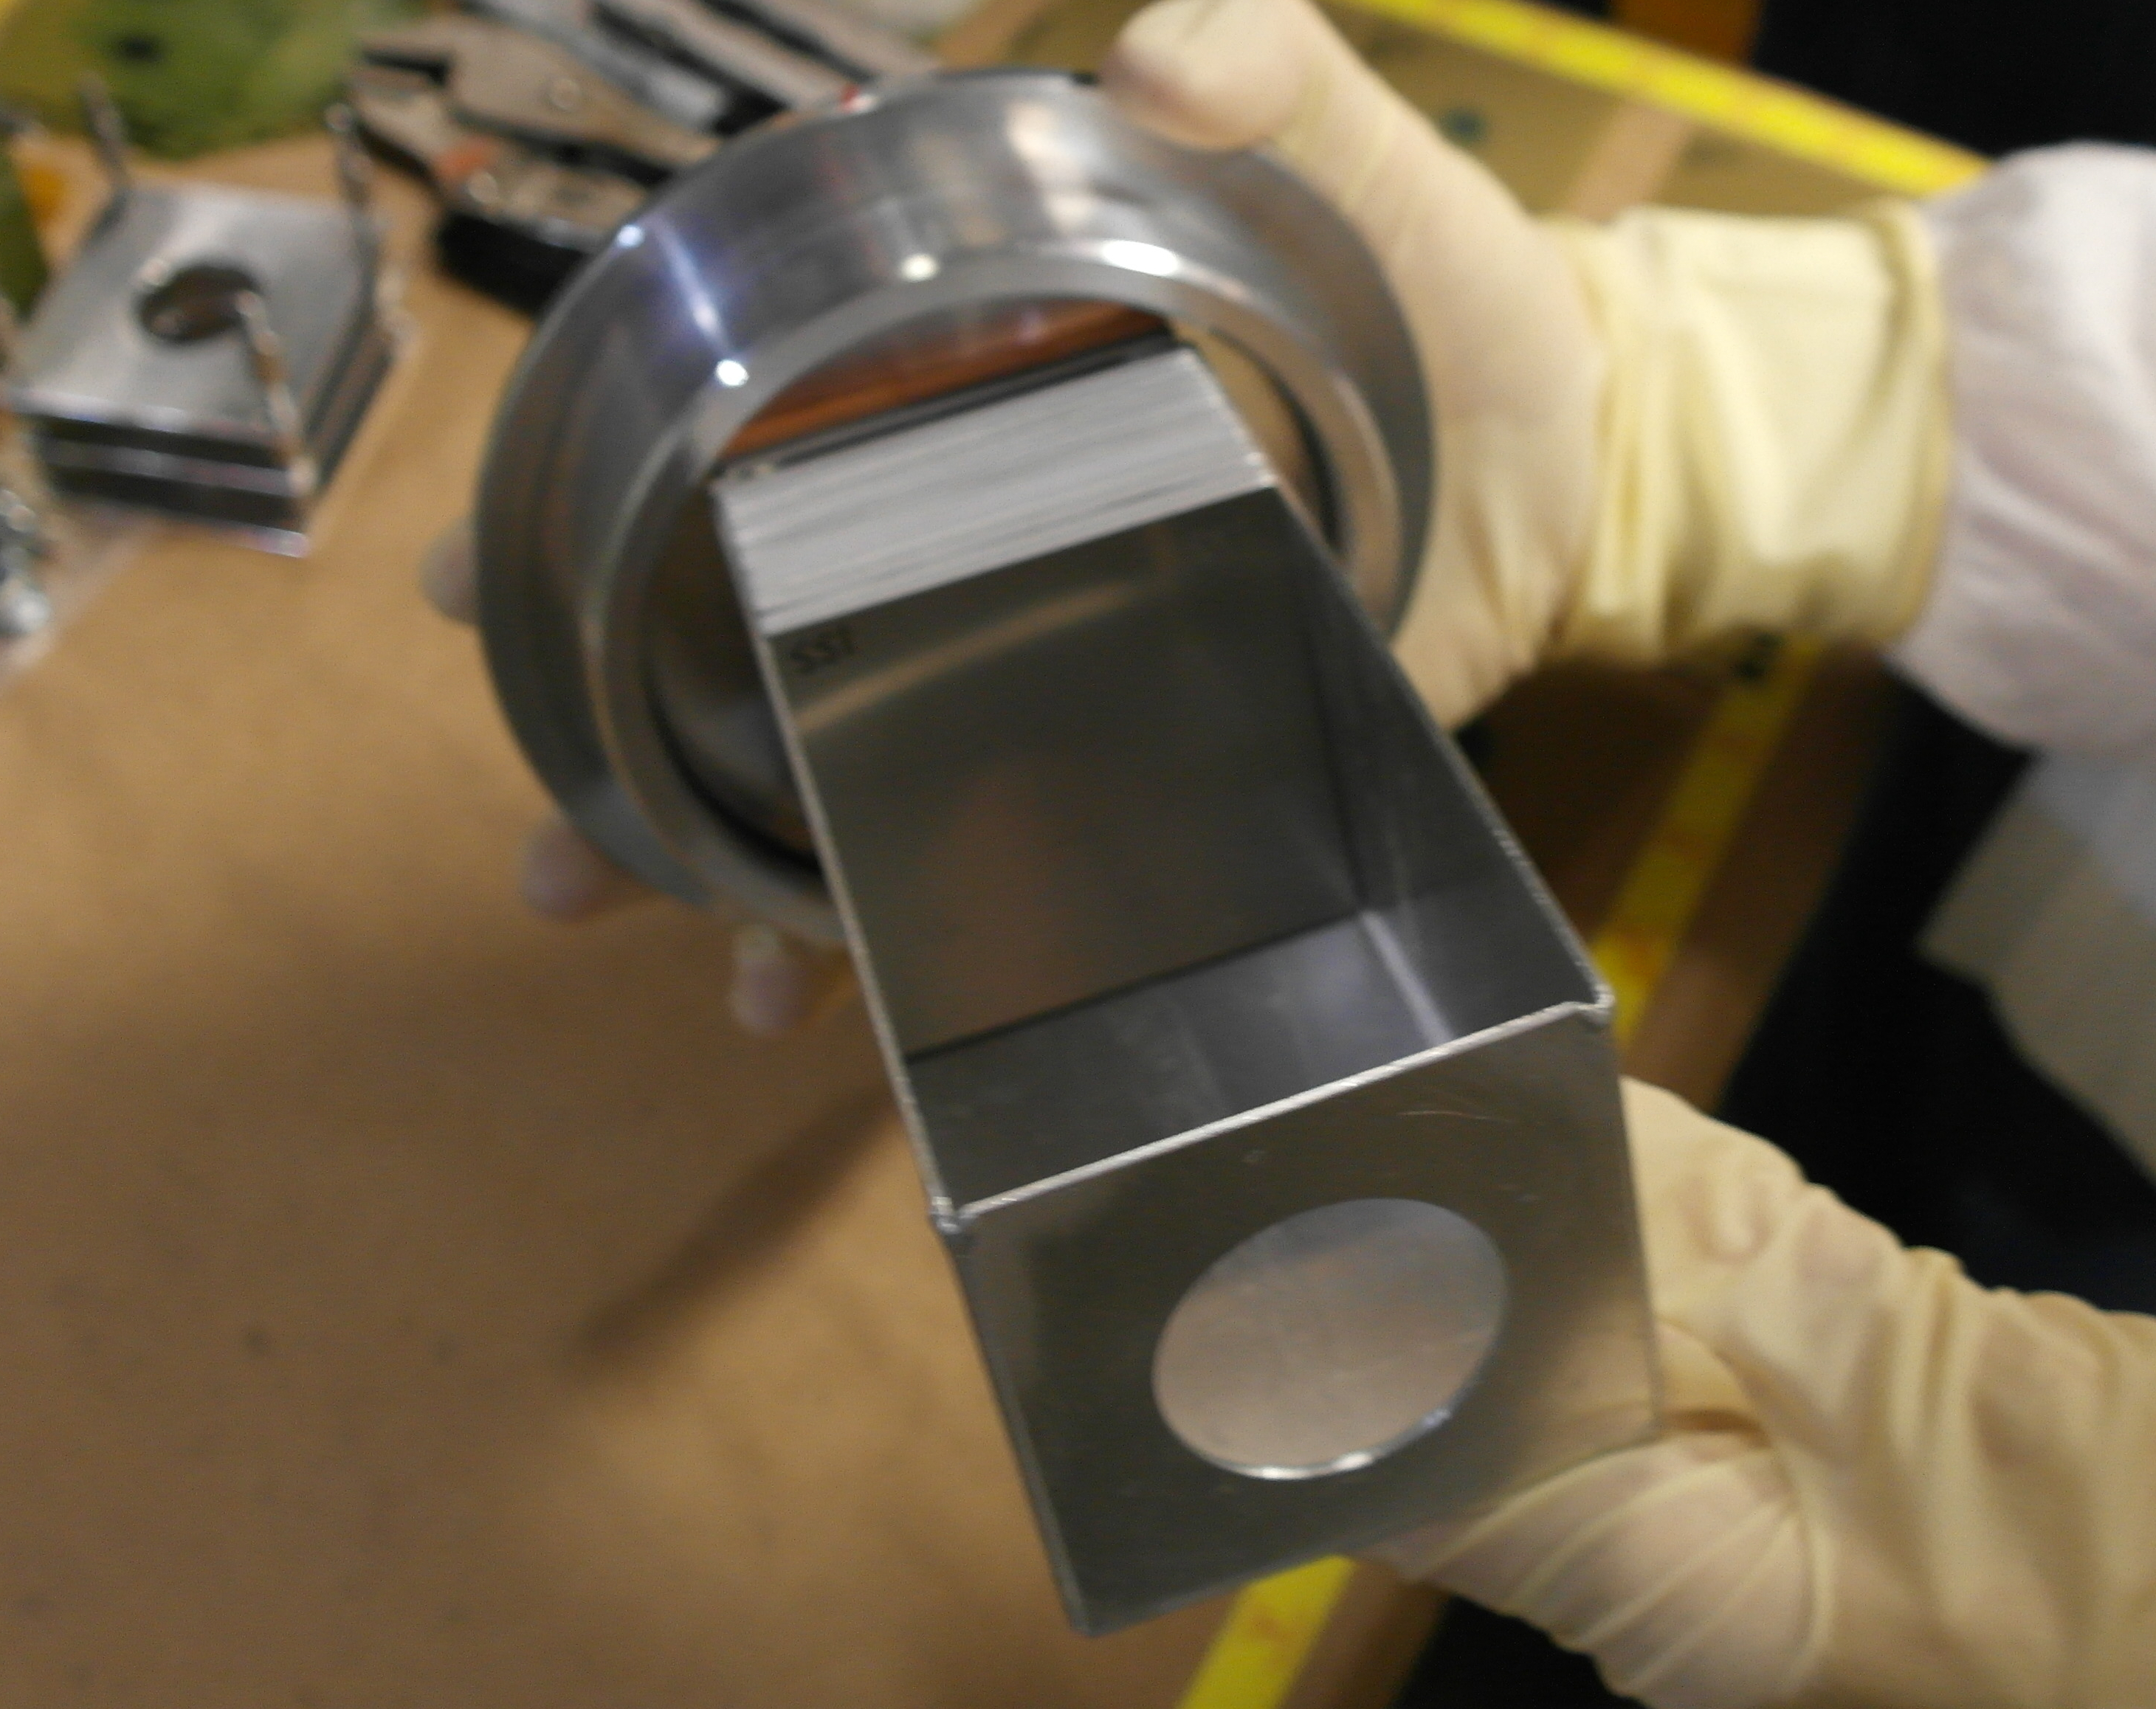
\includegraphics[width=0.5\linewidth]{./figures/SAM_2494.JPG}
 % IMG_1975.JPG: 3264x2448 pixel, 72dpi, 115.15x86.36 cm, bb=0 0 3264 2448
 \caption{\label{fig:fe_target_stack}Photograph of the assembled 25\,MeV target stack, before it was mounted in the beamline. The proton beam enters through the circular entrance in the foreground, and the upstream stainless steel profile monitor (SS-5) is visible at the front of the stack.}
\end{figure}

% Separate tables
% 
% % Please add the following required packages to your document preamble:
% % \usepackage{booktabs}
% \begin{table}
% \centering
% \caption{Specifications of the  target stack design in the present work. The proton beam enters the stack upstream of the 249.8 \mmicro m SS profile monitor, and is transported through the stack in the order presented here. The 6061 aluminum degraders have a measured density of approximately 2.80 g/cm$^3$. Their areal densities were determined using the variance minimization techniques described  in this work  and the earlier paper by Graves \etal\ \cite{Graves2016}. At both the front and rear of the target stack's foils, a 316 stainless steel foil is inserted to serve as a beam profile monitor --- after end-of-bombardment (EoB), decay radiation emitted from these activated stainless steel foils were used to develop radiochromic film (Gafchromic EBT3), revealing the spatial profile of the beam entering and exiting the stack.}
% \label{tab:fe_stack_table}
% \small
% \begin{tabular}{@{}llll@{}}
% \toprule
% % Target Layer       & Nominal Thickness & Measured thickness (mg/cm\textasciicircum 2) & Thickness Uncertainty (\%) \\ \midrule
% Target layer       & \begin{tabular}[c]{@{}l@{}}Measured \\ thickness\end{tabular} & \begin{tabular}[c]{@{}l@{}}Measured areal\\density (mg/cm$^2$)\end{tabular} & \begin{tabular}[c]{@{}l@{}}Areal density \\ uncertainty (\%)\end{tabular} \\ \midrule
% SS profile monitor SS-5 & 130.94 \mmicro m                                              & 100.57                                                                      & 0.17                                                                      \\
% Fe-08                   & 26.25 \mmicro m                                               & 19.69                                                                       & 0.17                                                                      \\
% Ti-14                   & 25.01 \mmicro m                                               & 10.87                                                                       & 0.36                                                                      \\
% Cu-14                   & 24.01 \mmicro m                                               & 17.49                                                                       & 0.40                                                                      \\
% Al Degrader E-09        & 256.5 \mmicro m                                               & --                                                                          & --                                                                        \\
% Fe-09                   & 26.5 \mmicro m                                                & 19.90                                                                       & 0.09                                                                      \\
% Ti-15                   & 23.81 \mmicro m                                               & 10.97                                                                       & 0.11                                                                      \\
% Cu-15                   & 21.81 \mmicro m                                               & 17.63                                                                       & 0.46                                                                      \\
% Al Degrader H-01        & 127.49 \mmicro m                                              & --                                                                          & --                                                                        \\
% Fe-10                   & 26.5 \mmicro m                                                & 19.84                                                                       & 0.11                                                                      \\
% Ti-16                   & 24.6 \mmicro m                                                & 10.96                                                                       & 0.32                                                                      \\
% Cu-16                   & 22.01 \mmicro m                                               & 17.22                                                                       & 0.25                                                                      \\
% Fe-11                   & 27.26 \mmicro m                                               & 19.96                                                                       & 0.17                                                                      \\
% Ti-17                   & 25.01 \mmicro m                                               & 10.88                                                                       & 0.25                                                                      \\
% Cu-17                   & 29 \mmicro m                                                  & 21.91                                                                       & 0.33                                                                      \\
% Fe-12                   & 27.01 \mmicro m                                               & 20.03                                                                       & 0.12                                                                      \\
% Ti-18                   & 25.01 \mmicro m                                               & 11.00                                                                       & 0.87                                                                      \\
% Cu-18                   & 28.75 \mmicro m                                               & 22.33                                                                       & 0.14                                                                      \\
% Fe-013                  & 26.25 \mmicro m                                               & 20.05                                                                       & 0.16                                                                      \\
% Ti-19                   & 26.6 \mmicro m                                                & 11.01                                                                       & 0.22                                                                      \\
% Cu-19                   & 28.75 \mmicro m                                               & 22.32                                                                       & 0.19                                                                      \\
% Fe-14                   & 25.75 \mmicro m                                               & 20.11                                                                       & 0.19                                                                      \\
% Ti-20                   & 27.01 \mmicro m                                               & 11.06                                                                       & 0.35                                                                      \\
% Cu-20                   & 28.26 \mmicro m                                               & 22.34                                                                       & 0.28                                                                      \\
% SS profile monitor SS-6 & 131.5 \mmicro m                                               & 100.99                                                                      & 0.17                                                                      \\
%  \bottomrule
% \end{tabular}
% \end{table}
% 
% 
% 
% 
% % Please add the following required packages to your document preamble:
% % \usepackage{booktabs}
% \begin{table}
% \centering
% \caption{Specifications of the  target stack design in the present work. The proton beam enters the stack upstream of the 249.8 \mmicro m SS profile monitor, and is transported through the stack in the order presented here. The 6061 aluminum degraders have a measured density of approximately 2.80 g/cm$^3$. Their areal densities were determined using the variance minimization techniques described  in this work  and the earlier paper by Graves \etal\ \cite{Graves2016}. At both the front and rear of the target stack's foils, a 316 stainless steel foil is inserted to serve as a beam profile monitor --- after end-of-bombardment (EoB), decay radiation emitted from these activated stainless steel foils were used to develop radiochromic film (Gafchromic EBT3), revealing the spatial profile of the beam entering and exiting the stack.}
% \label{tab:fe_stack_table2}
% \small
% \begin{tabular}{@{}llll@{}}
% \toprule
% % Target Layer       & Nominal Thickness & Measured thickness (mg/cm\textasciicircum 2) & Thickness Uncertainty (\%) \\ \midrule
% Target layer       & \begin{tabular}[c]{@{}l@{}}Measured \\ thickness\end{tabular} & \begin{tabular}[c]{@{}l@{}}Measured areal\\density (mg/cm$^2$)\end{tabular} & \begin{tabular}[c]{@{}l@{}}Areal density \\ uncertainty (\%)\end{tabular} \\ \midrule
% SS profile monitor SS-3 & 130.9 \mmicro m                                               & 100.48                                                                      & 0.17                                                                      \\
% Fe-01                   & 25.75 \mmicro m                                               & 20.22                                                                       & 0.21                                                                      \\
% Ti-01                   & 25.88 \mmicro m                                               & 11.09                                                                       & 0.16                                                                      \\
% Cu-01                   & 28.81 \mmicro m                                               & 22.40                                                                       & 0.11                                                                      \\
% Al Degrader A-1         & 2.24 mm                                                       & --                                                                          & --                                                                        \\
% Fe-02                   & 25.5 \mmicro m                                                & 19.91                                                                       & 0.13                                                                      \\
% Ti-02                   & 25.74 \mmicro m                                               & 10.94                                                                       & 0.24                                                                      \\
% Cu-02                   & 28.75 \mmicro m                                               & 22.32                                                                       & 0.40                                                                      \\
% Al Degrader A-2         & 2.24 mm                                                       & --                                                                          & --                                                                        \\
% Fe-03                   & 25.25 \mmicro m                                               & 20.00                                                                       & 0.27                                                                      \\
% Ti-03                   & 25.91 \mmicro m                                               & 11.25                                                                       & 0.15                                                                      \\
% Cu-03                   & 28.86 \mmicro m                                               & 22.49                                                                       & 0.20                                                                      \\
% Al Degrader C-1         & 0.97 mm                                                       & --                                                                          & --                                                                        \\
% Fe-04                   & 25.25 \mmicro m                                               & 19.93                                                                       & 0.33                                                                      \\
% Ti-04                   & 25.84 \mmicro m                                               & 10.91                                                                       & 0.18                                                                      \\
% Cu-04                   & 28.78 \mmicro m                                               & 22.38                                                                       & 0.29                                                                      \\
% Al Degrader C-2         & 0.97 mm                                                       & --                                                                          & --                                                                        \\
% Fe-05                   & 25.64 \mmicro m                                               & 20.02                                                                       & 0.24                                                                      \\
% Ti-05                   & 25.86 \mmicro m                                               & 10.99                                                                       & 0.30                                                                      \\
% Cu-05                   & 28.77 \mmicro m                                               & 22.35                                                                       & 0.12                                                                      \\
% Al Degrader C-3         & 0.97 mm                                                       & --                                                                          & --                                                                        \\
% Fe-06                   & 25.75 \mmicro m                                               & 20.21                                                                       & 0.26                                                                      \\
% Ti-06                   & 25.5 \mmicro m                                                & 11.15                                                                       & 0.23                                                                      \\
% Cu-06                   & 28.83 \mmicro m                                               & 22.43                                                                       & 0.10                                                                      \\
% Al Degrader C-4         & 0.97 mm                                                       & --                                                                          & --                                                                        \\
% Fe-07                   & 25.76 \mmicro m                                               & 19.93                                                                       & 0.19                                                                      \\
% Ti-07                   & 25.75 \mmicro m                                               & 11.17                                                                       & 0.33                                                                      \\
% Cu-07                   & 28.76 \mmicro m                                               & 22.34                                                                       & 0.24                                                                      \\
% Al Degrader H-02        & 127.04 \mmicro m                                              & 34.51                                                                       & 0.20                                                                      \\
% SS profile monitor SS-4 & 131.21 \mmicro m                                              & 101.25                                                                      & 0.16                                                                     \\
%  \bottomrule
% \end{tabular}
% \end{table}

% Combined table
% Please add the following required packages to your document preamble:
% \usepackage{booktabs}
\begin{table}
\centering
\caption{Specifications of the 25\,MeV and 55\,MeV target stack designs in the present work. The proton beam enters the stack upstream of the SS-5 and SS-3 profile monitors, respectively, and is transported through the stack in the order presented here. The 6061 aluminum degraders have a measured density of approximately 2.69 g/cm$^3$. Their areal densities were determined using the variance minimization techniques described  in this work  and our earlier paper \cite{Voyles2018a}. 
% the earlier paper by Graves \etal\ \cite{Graves2016}.
A 316 stainless steel foil is inserted at both the front and rear of each target stack as a monitor of the beam's spatial profile, by developing radiochromic film (Gafchromic EBT3) after end-of-bombardment (EoB).}
\label{tab:fe_stack_table}
\small
\resizebox{\textwidth}{!}{%
\begin{tabular}{@{}llll|llll@{}}
\toprule
% Target Layer       & Nominal Thickness & Measured thickness (mg/cm\textasciicircum 2) & Thickness Uncertainty (\%) \\ \midrule
25\,MeV Target layer            & \begin{tabular}[c]{@{}l@{}}Measured \\ thickness\end{tabular} & \begin{tabular}[c]{@{}l@{}}Measured\\areal density\\(mg/cm$^2$)\end{tabular} & \begin{tabular}[c]{@{}l@{}}Uncertainty \\ in areal\\ density  (\%)\end{tabular} & 55\,MeV Target layer            & \begin{tabular}[c]{@{}l@{}}Measured \\ thickness\end{tabular} & \begin{tabular}[c]{@{}l@{}}Measured\\areal density\\(mg/cm$^2$)\end{tabular} & \begin{tabular}[c]{@{}l@{}}Uncertainty \\ in areal\\ density  (\%)\end{tabular} \\
\midrule
SS profile monitor SS-5 & 130.94 \mmicro m                                              & 100.57                                                                      & 0.17                                                                      & SS profile monitor SS-3 & 130.9 \mmicro m                                               & 100.48                                                                      & 0.17                                                                      \\
Fe-08                   & 26.25 \mmicro m                                               & 19.69                                                                       & 0.17                                                                      & Fe-01                   & 25.75 \mmicro m                                               & 20.22                                                                       & 0.21                                                                      \\
Ti-14                   & 25.01 \mmicro m                                               & 10.87                                                                       & 0.36                                                                      & Ti-01                   & 25.88 \mmicro m                                               & 11.09                                                                       & 0.16                                                                      \\
Cu-14                   & 24.01 \mmicro m                                               & 17.49                                                                       & 0.40                                                                      & Cu-01                   & 28.81 \mmicro m                                               & 22.40                                                                       & 0.11                                                                      \\
Al Degrader E-09        & 256.5 \mmicro m                                               & --                                                                          & --                                                                        & Al Degrader A-1         & 2.24 mm                                                       & --                                                                          & --                                                                        \\
Fe-09                   & 26.5 \mmicro m                                                & 19.90                                                                       & 0.09                                                                      & Fe-02                   & 25.5 \mmicro m                                                & 19.91                                                                       & 0.13                                                                      \\
Ti-15                   & 23.81 \mmicro m                                               & 10.97                                                                       & 0.11                                                                      & Ti-02                   & 25.74 \mmicro m                                               & 10.94                                                                       & 0.24                                                                      \\
Cu-15                   & 21.81 \mmicro m                                               & 17.63                                                                       & 0.46                                                                      & Cu-02                   & 28.75 \mmicro m                                               & 22.32                                                                       & 0.40                                                                      \\
Al Degrader H-01        & 127.09 \mmicro m                                              & --                                                                          & --                                                                        & Al Degrader A-2         & 2.24 mm                                                       & --                                                                          & --                                                                        \\
Fe-10                   & 26.5 \mmicro m                                                & 19.84                                                                       & 0.11                                                                      & Fe-03                   & 25.25 \mmicro m                                               & 20.00                                                                       & 0.27                                                                      \\
Ti-16                   & 24.6 \mmicro m                                                & 10.96                                                                       & 0.32                                                                      & Ti-03                   & 25.91 \mmicro m                                               & 11.25                                                                       & 0.15                                                                      \\
Cu-16                   & 22.01 \mmicro m                                               & 17.22                                                                       & 0.25                                                                      & Cu-03                   & 28.86 \mmicro m                                               & 22.49                                                                       & 0.20                                                                      \\
Fe-11                   & 27.26 \mmicro m                                               & 19.96                                                                       & 0.17                                                                      & Al Degrader C-1         & 0.97 mm                                                       & --                                                                          & --                                                                        \\
Ti-17                   & 25.01 \mmicro m                                               & 10.88                                                                       & 0.25                                                                      & Fe-04                   & 25.25 \mmicro m                                               & 19.93                                                                       & 0.33                                                                      \\
Cu-17                   & 29 \mmicro m                                                  & 21.91                                                                       & 0.33                                                                      & Ti-04                   & 25.84 \mmicro m                                               & 10.91                                                                       & 0.18                                                                      \\
Fe-12                   & 27.01 \mmicro m                                               & 20.03                                                                       & 0.12                                                                      & Cu-04                   & 28.78 \mmicro m                                               & 22.38                                                                       & 0.29                                                                      \\
Ti-18                   & 25.01 \mmicro m                                               & 11.00                                                                       & 0.87                                                                      & Al Degrader C-2         & 0.97 mm                                                       & --                                                                          & --                                                                        \\
Cu-18                   & 28.75 \mmicro m                                               & 22.33                                                                       & 0.14                                                                      & Fe-05                   & 25.64 \mmicro m                                               & 20.02                                                                       & 0.24                                                                      \\
Fe-13                  & 26.25 \mmicro m                                               & 20.05                                                                       & 0.16                                                                      & Ti-05                   & 25.86 \mmicro m                                               & 10.99                                                                       & 0.30                                                                      \\
Ti-19                   & 26.6 \mmicro m                                                & 11.01                                                                       & 0.22                                                                      & Cu-05                   & 28.77 \mmicro m                                               & 22.35                                                                       & 0.12                                                                      \\
Cu-19                   & 28.75 \mmicro m                                               & 22.32                                                                       & 0.19                                                                      & Al Degrader C-3         & 0.97 mm                                                       & --                                                                          & --                                                                        \\
Fe-14                   & 25.75 \mmicro m                                               & 20.11                                                                       & 0.19                                                                      & Fe-06                   & 25.75 \mmicro m                                               & 20.21                                                                       & 0.26                                                                      \\
Ti-20                   & 27.01 \mmicro m                                               & 11.06                                                                       & 0.35                                                                      & Ti-06                   & 25.5 \mmicro m                                                & 11.15                                                                       & 0.23                                                                      \\
Cu-20                   & 28.26 \mmicro m                                               & 22.34                                                                       & 0.28                                                                      & Cu-06                   & 28.83 \mmicro m                                               & 22.43                                                                       & 0.10                                                                      \\
SS profile monitor SS-6 & 131.5 \mmicro m                                               & 100.99                                                                      & 0.17                                                                      & Al Degrader C-4         & 0.97 mm                                                       & --                                                                          & --                                                                        \\
                        &                                                               &                                                                             &                                                                           & Fe-07                   & 25.76 \mmicro m                                               & 19.93                                                                       & 0.19                                                                      \\
                        &                                                               &                                                                             &                                                                           & Ti-07                   & 25.75 \mmicro m                                               & 11.17                                                                       & 0.33                                                                      \\
                        &                                                               &                                                                             &                                                                           & Cu-07                   & 28.76 \mmicro m                                               & 22.34                                                                       & 0.24                                                                      \\
                        &                                                               &                                                                             &                                                                           & Al Degrader H-02        & 127.04 \mmicro m                                              & --\cmmnt{34.51}                                                                       & --\cmmnt{0.20}                                                                      \\
                        &                                                               &                                                                             &                                                                           & SS profile monitor SS-4 & 131.21 \mmicro m                                              & 101.25                                                                      & 0.16                                                                     \\
 \bottomrule
\end{tabular}
}
\end{table}


Both target stacks were assembled and separately irradiated at the  Lawrence Berkeley National Laboratory  (LBNL), using the 88-Inch Cyclotron, a  K=140 sector-focused cyclotron.
The 25\,MeV stack was irradiated for approximately 20\,minutes with a nominal current of 100\,nA,  for an anticipated integral current of 31.61\,nAh. 
The 55\,MeV stack was irradiated for approximately 10\,minutes with a nominal current of 120\,nA,  for an anticipated integral current of 20.78\,nAh. 
The beam current, measured using a current integrator on the electrically-isolated beamline, remained stable under these conditions for the duration of each irradiation.
The proton beam incident upon each stack's upstream stainless steel profile monitor had a maximum energy of either 25 or 55\,MeV, with an approximately 2\% energy width due to multi-turn extraction --- these energy profiles were used for all later analysis.
Following end-of-bombardment (EoB), each stack was removed from the beamline and disassembled.
All activated foils were transported to a counting lab for gamma spectrometry, which started approximately 30\,minutes following the end of each irradiation.




% The \texttt{widetext} environment will make the text the width of the
% full page, as on page~\pageref{eq:wideeq}. (Note the use the
% \verb+\pageref{#1}+ command to refer to the page number.) 
% \paragraph{Note (Fourth-level head is run in)}
% The width-changing commands only take effect in two-column formatting. 
% There is no effect if text is in a single column.

\subsection{\label{sec:spectroscopy_fe}Quantification of induced activities}

% \comment{Get detector specs from Alex}

% For consistency, a
A single detector was used in this measurement, an ORTEC GMX Series (model \#GMX-50220-S)  High-Purity Germanium (HPGe) detector.
The detector is a nitrogen-cooled coaxial n-type HPGe with a 0.5\,mm beryllium window, and a 64.9\,mm diameter, 57.8\,mm long crystal.
Samples were counted at fixed positions ranging 5--60  cm (5\% maximum permissible dead-time) from the front face of the detector, with a series of standard calibration sources used to determine energy and efficiency for each position.
The foils were counted  for a period of 4 weeks following end-of-bombardment (EoB), to accurately quantify all induced activities.
An example of one of the gamma-ray spectra collected in such a fashion is shown in \autoref{fig:gspec_femn}.
% An example of one of the gamma-ray spectra collected in such a fashion is shown in \autoref{fig:gspec}.
For all spectra collected, net peak areas were fitted using the gamma spectrometry analysis code FitzPeaks \cite{fitzgerald2009fitzpeaks}, which utilizes the SAMPO fitting algorithms for gamma ray spectra \cite{Aarnio2001}.
% , which has been shown to perform best in comparisons with other common analysis codes \cite{Jackman2014}.
%, due to its peak fitting algorithms and incorporation  of calibrated detector-specific peak shapes and widths. 



% Following  acquisition, the decaying product nuclei corresponding to each observed peak in the collected spectra were identified.
The net  counts in each fitted gamma-ray photopeak were converted into  activities for the decaying  activation products, using calibrated detector efficiencies and gamma-ray intensities for each transition.
% and  corrections for gamma-ray attenuation within each foil packet
% The calibrated detector efficiencies, along with gamma-ray intensities for each transition and  corrections for gamma-ray attenuation within each foil packet, were used to convert the net  counts in each fitted gamma-ray photopeak into an activity for the decay of the activation products.  
The nuclear decay data used in this work is tabulated, for reference, in \autoref{tab:fe_nudat_table_monitors} and \autoref{tab:fe_nudat_table_nb} of Appendix \ref{sec:fe_data}.
Corrections for gamma-ray attenuation within each foil packet were made, using  photon attenuation coefficients from the XCOM photon cross sections database  \cite{berger2011xcom}.
% As nearly all of the product nuclei have multiple high-intensity gamma-rays, decay gamma-rays from the product nuclei were measured at multiple points in time (up to 2 weeks after EoB), as well as multiple independent activity measurements at each time point, based on each of its observed gamma-rays.
% Decay gamma-rays from the product nuclei were measured at multiple points in time (up to 2 weeks after EoB), and as nearly all of the product nuclei have multiple high-intensity gamma-rays, this provided independent activity measurements at each time point.
% activity for each gamma-ray possesses a 
The total propagated uncertainty in  activity is the quadrature sum of the uncertainty in  fitted peak areas, uncertainty in detector efficiency calibration, and uncertainty in the gamma-ray branching ratio data.




As in our previous work, these activities used to calculate cross sections, and are differentiated between cumulative and independent \cite{Voyles2018a}.
For the first observable product nuclei in a mass chain, its (p,x) cross section will be reported as a cumulative cross section ($\sigma_c$), which is the sum of direct production of that nucleus, as well as decay of its  precursors and any other independent cross sections leading to that nucleus. 
% In addition, 
Cumulative cross sections will be reported whenever it is impossible to use decay spectrometry to distinguish independent production of a nucleus from decay feeding.
For all remaining observed reaction products in the mass chain, and cases where no decay precursors exist, independent cross sections ($\sigma_i$) will be reported, allowing for determination of the independent production via subtraction  and facilitating comparison to reaction model calculations.  
Solutions to the first- and higher-order  Bateman equations are used for separation of  feeding contributions from decay precursors, that  independent cross sections may be reported \cite{bateman1910solution,Cetnar2006}.



\begin{figure}
 \centering
 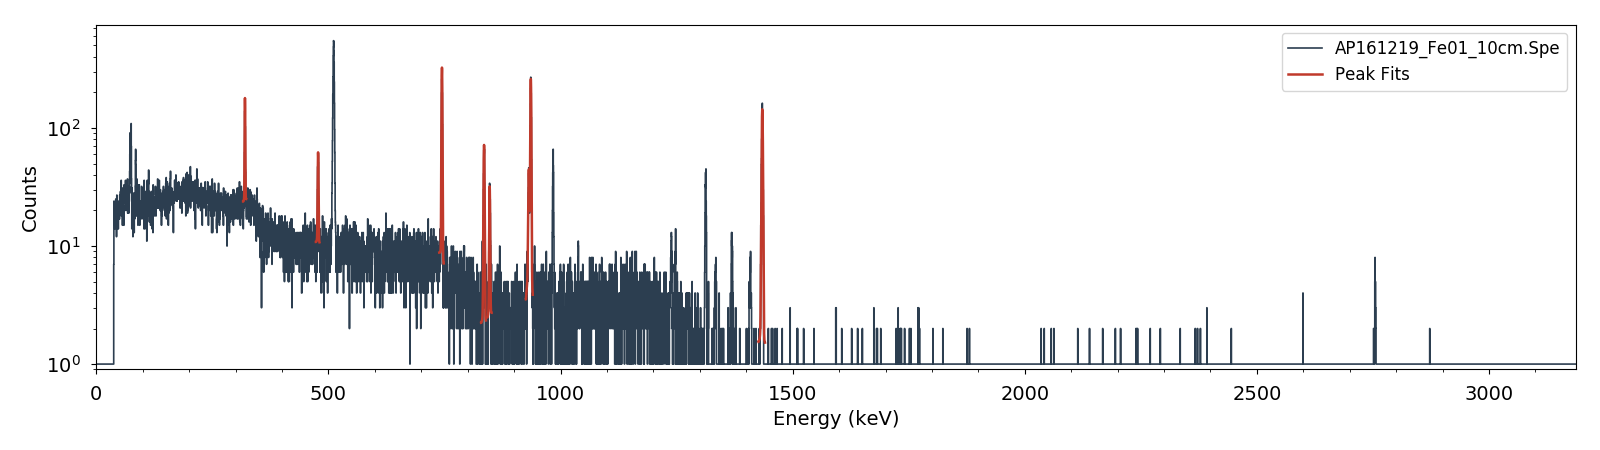
\includegraphics[width=6in]{./figures/AP161219_Fe01_10cm.png}
 % sample_gspec.pdf: 489x257 pixel, 72dpi, 17.25x9.07 cm, bb=0 0 489 257
 \caption{\textred{Replace this figure!!!}  A gamma spectrum collected from an activated Fe foil at approximately \textred{80 MeV}. While the majority of observed reaction products are visible in this spectrum,  the \ce{^{51}Cr}, \ce{^{52m}Mn}, and \ce{^{52g}Mn} decay lines, which form the   primary reaction channels of interest, are  clearly isolated from surrounding peaks.}
 \label{fig:gspec_femn}
\end{figure}



% Since many of the reaction products populated by energetic protons are more than one decay off of stability, many of these are produced not only  directly by reactions, but also indirectly by decay down a mass chain.
% To this end, it is useful to differentiate between the types of cross sections reported in this work. 
% For the first observable product nuclei in a mass chain, its (p,x) cross section will be reported as a cumulative cross section ($\sigma_c$), which is the sum of direct production of that nucleus, as well as decay of its  precursors and any other independent cross sections leading to that nucleus. 
% % In addition, 
% Cumulative cross sections will be reported whenever it is impossible to use decay spectrometry to distinguish independent production of a nucleus from decay feeding.
% For all remaining observed reaction products in the mass chain, and cases where no decay precursors exist, independent cross sections ($\sigma_i$) will be reported, allowing for determination of the independent production via subtraction  and facilitating comparison to reaction model calculations.  
% 
% 
% 
% % To convert these activities into cross sections, c
% Corrections must be made for the decay of the various reaction products during the time between EoB and the spectrum acquisition, in order to calculate $A_0$, the initial activity at EoB, from the measured activities.
% The use of  multiple gamma-rays at multiple points after EoB to calculate initial activities  for each observed product nucleus allows for a more accurate  determination of $A_0$ than simply basing its calculation off of a single gamma-ray observation.
% For the case of cumulative cross sections, EoB activities were quantified by fitting the activities observed at multiple time points $t$ (since EoB) to the well-known radioactive decay law.
% % \begin{equation}
% % A\pp{t} = A_0 e^{-\lambda t}
% % \end{equation}
% Nonlinear regression was used for this fitting process, minimizing on $\chi^2$\,/\,degree of freedom, so that not only would the uncertainty-weighted EoB activities be fitted, but that a 1-$\sigma$ confidence interval in $A_0$ could be reported as as well.
% As with the gamma-ray intensities, all lifetimes used in this work are tabulated in \autoref{tab:fe_nudat_table_monitors} and \autoref{tab:fe_nudat_table_nb} of \ref{sec:fe_data}.
% In the case of independent cross sections, a similar process was followed, quantifying $A_i\pp{t=0} = A_{i,0}$, the EoB activity of nuclide $i$, by instead regressing to the solutions to the Bateman equation \cite{bateman1910solution,Cetnar2006}:
% \begin{equation}
% A_n\pp{t} = \lambda_n \sum_{i=1}^n \left[  N_{i,0} \times \pp{\prod_{j=i}^{n-1}\lambda_j} \times \pp{\sum_{j=i}^n \dfrac{e^{-\lambda_j t}}{\prod_{i\neq j}^n \pp{\lambda_i - \lambda_j}}  }   \right]
% \end{equation}
% where $j$ refers to a precursor nucleus populating a specific end-product.  
% While higher-order terms were added if needed, typically for an isomeric state in a particular mass chain,  the second-order expansion ($n=2$) was often sufficient to quantify EoB activities in a mass chain, simplifying to:
% \begin{equation}
% A_2\pp{t} = \dfrac{A_{1,0}\lambda_2}{\lambda_1 - \lambda_2} \pp{e^{-\lambda_2 t} - e^{-\lambda_1 t}} + A_{2,0} e^{-\lambda_2 t}
% \end{equation}
% In these cases, the previously-quantified EoB activities from decay precursors ($A_{1,0}$, etc) would be substituted in, so that the feeding contributions from decay could be separated and an independent cross section reported.
% After quantifying the cumulative EoB activities at the top of a mass chain and all subsequent independent EoB activities, these will be later used to report the various cross sections for all observed reaction products and isomeric states. 





% A citation in text uses the command \verb+\cite{#1}+ or
% \verb+\onlinecite{#1}+ and refers to an entry in the bibliography. 
% An entry in the bibliography is a reference to another document.

\subsection{\label{sec:dosimetry_fe}Proton fluence determination}


In addition to the stack's overall beam current measurements using  beamline current integrators, thin \ce{^{nat}Ti} and \ce{^{nat}Cu} foils were included along with the \ce{^{nat}Fe} targets at each energy position, to monitor beam current at each position within the stack.
% These foils have been recommended for use as proton monitor foils in the 30 \textless\ E$_\text{p}$ \textless\ 100 MeV regime by the IAEA, as the
The IAEA-recommended \ce{^{nat}Ti}(p,x)\ce{^{46}Sc}, \ce{^{nat}Ti}(p,x)\ce{^{48}V},  \ce{^{nat}Cu}(p,x)\ce{^{62}Zn}, and \ce{^{nat}Cu}(p,x)\ce{^{63}Zn} monitor reactions were used for  proton fluence measurement 
% , using values  
% and uncertainties 
% from the 2017 IAEA re-evaluation  
\cite{Hermanne2018}.
% The recommended cross section values for each of these reactions were used in all calculations of proton fluence for the above monitor reactions.
As in our previous work, the integral form of the well-known activation equation was used to  determine proton fluence ($I \Delta t $),
% in each monitor foil
in order to account for energy loss across each monitor foil:
\begin{equation}
I \Delta t = \dfrac{A_0 \Delta t}{\rho \Delta r \pp{1-e^{-\lambda \Delta t}} \int \sigma\pp{E} \dfrac{d\phi}{dE} dE}
\end{equation}
The propagated uncertainty in proton fluence is calculated as the quadrature sum of (1) the uncertainty in quantified EoB activity, (2) uncertainty in the duration of irradiation (conservatively estimated at 60 s, to account for any transient changes in beam current), (3) uncertainty in foil areal density, (4) uncertainty in monitor product half-life (included, but normally negligible), (5) uncertainty in IAEA recommended cross section (using values  from the 2017 IAEA re-evaluation  \cite{Hermanne2018}), and (6) uncertainty in differential proton fluence (from transport simulations).





% Because REV\TeX\ uses the \verb+natbib+ package of Patrick Daly, 
% the entire repertoire of commands in that package are available for your document;
% see the \verb+natbib+ documentation for further details. Please note that
% REV\TeX\ requires version 8.31a or later of \verb+natbib+.

\subsection{\label{sec:proton_transport_fe}Proton transport calculations}

Estimates of the proton beam energy for preliminary stack designs were calculated using the Anderson \& Ziegler (A\&Z) stopping power formalism \cite{Andersen_Ziegler_1977,Ziegler1985,Ziegler1999}.
However, the more rigorous Monte Carlo N-Particle transport code MCNP6.1 was used for simulation of the full 3-D target stack, to determine the full proton energy and fluence distribution for each foil   \cite{Goorley2012}. 
$10^8$ source protons were used for all MCNP simulations, which places the statistical uncertainty in proton energy distributions at less than 0.01\%.
As with the determination of proton fluence in monitor foils, the progressively increasing energy straggle towards the rear of each stack is accounted for using the differential proton fluence from MCNP simulation of proton transport.
These energy distributions $\frac{d\phi}{dE}$ are used to calculate a flux-weighted average proton  energy $\langle E \rangle$, which accounts for the slowing-down of protons within a foil (particularly in the low-energy stack) and reports the effective  energy centroid for each foil:
\begin{equation}
\langle E \rangle = \dfrac{{\displaystyle\int E \dfrac{d\phi}{dE} dE}}{{\displaystyle\int \dfrac{d\phi}{dE} dE}}
\end{equation}
To report a complete description of the representative energy for each foil, a bin width is provided through the  energy uncertainty, calculated as the full width at half maximum (FWHM) of the MCNP6-modeled energy distribution for each foil.


To correct for a spread in the apparent proton fluence, seen most strongly in rear stack positions, the \enquote{variance minimization} techniques utilized in our recent work and established by Graves \etal\ have been used to reduce uncertainty in proton fluence assignments \cite{Voyles2018a,Graves2016}.
This method is based on the assumption that the independent measurements of proton fluence from the different monitor reactions used in this work should all be consistent at each energy position.
Assuming that the recommended monitor reaction cross sections and MCNP6-modeled energy distributions are both accurate, residual disagreement in the  observed proton fluences is thus primarily due to poorly characterized stopping power in simulations, or a systematic error in the 
% stack design, namely, the
areal densities of the stack components. 
This disagreement is minor at the front of the stack, and gets progressively worse as the beam is degraded, due to the compounded effect of systematic uncertainties in stack areal densities.



When performing  a variance minimization, it is important to apply this variation of effective areal density  to the stack components which  have the most significant impact on beam degradation, as any systematic error in the areal densities used for these components will cause a disagreement in the observed fluences.
For the 55\,MeV stack, the aluminum degraders are used for variance minimization, as they make up more than 80\% of the areal density of the stack, and this play the largest role in beam degradation.
% 
% Update this post-results!
% 
% Delete  the paragraph break!
% 

\textred{Update this post-results!}
For the 25\,MeV stack, the Kapton tape was chosen for variance minimization, as the foil packets themselves are responsible for the majority of beam degradation.
While it only makes up approximately 20\% of the low-energy stack's areal density, the Kapton surrounding each foil packet has a greater areal density than the foil itself.
In addition, it is far easier to directly characterize the areal density of the metallic foils than it is for the Kapton, resulting in only an approximate value for the latter.
This is of relatively minor consequence for higher-energy irradiations (especially relative to any beam degraders), but the stopping power of the Kapton at this energy range may cause as much as a loss of 0.5\,MeV by the rear of this stack, making the precise areal density a source of significant uncertainty.




In performing the  minimization, the areal density of each of the  aluminum degraders (for the 55\,MeV stack)  were varied uniformly in MCNP6 simulations  by a factor of up to $\pm$25\% of nominal values, to find the effective density which minimized variance in the measured proton fluence at the lowest energy position (Ti-07, Cu-07).
For the 25\,MeV stack, the areal density of the E-09 and H-01 aluminum degraders was taken from that reached in the minimization of the 55\,MeV stack.
Using this value, the areal density of each of the  Kapton tape  layers  were likewise varied uniformly   by a factor of up to $\pm$25\% of nominal values, to find the effective density which minimized variance in the measured proton fluence at the next-to-lowest energy position (Ti-19, Cu-19).
These lowest energy positions were chosen as  minimization candidates, as they are the most sensitive to systematic uncertainties in stack design, due to the compounded effect of proton stopping powers.
In the 25\,MeV stack, activity was not seen in gamma spectrometry for the lowest-energy (Ti-20, Cu-20) monitor foils, implying that the beam was stopped at some point in between Fe-14 and Ti-20.
This observation is conclusive proof that  the true areal densities of the stack components differs from nominally measured values (primarily for the difficult-to-characterize Kapton tape), as transport calculations using nominal areal densities predict that the beam should exit the stack (at the SS-6 profile monitor) with an energy of approximately 7\,MeV.
As a result, this position was not used for minimization, with the Ti-19 and Cu-19 position being the lowest-energy reliable monitor foils in the stack.
The results of the minimization technique indicate a clear minimum in proton fluence variance for flux-weighted average \textred{41.34\,MeV} protons entering the last energy position of the 55\,MeV stack.
This is approximately \textred{2\,MeV} lower than the nominal MCNP6 simulations, and approximately \textred{3\,MeV} lower than nominal A\&Z calculations, both of which used the nominal 2.80\,g/cm$^3$ measured density of the  aluminum degraders.
This energy corresponds to an aluminum areal density of \textred{2.52\%} greater than nominal measurements, and serves as a lump correction for other minor systematic uncertainties in stack design, including stack areal densities and incident beam energy.
Similarly, for the 25\,Me stack, variance minimization converges on  flux-weighted average \textred{41.34\,MeV} protons entering the Fe-13/Ti-19/Cu-19 energy position, which is approximately \textred{2\,MeV} lower than the nominal MCNP6 simulations, and approximately \textred{3\,MeV} lower than nominal A\&Z calculations.
This energy corresponds to a Kapton tape areal density of \textred{2.52\%} greater than nominal measurements.
The impact of this variance minimization for improving disagreement in proton fluence is  clearly  seen in   \autoref{fig:fe_variance_mins}.




\begin{figure}
    \centering
    \subfloat{
        \centering
%         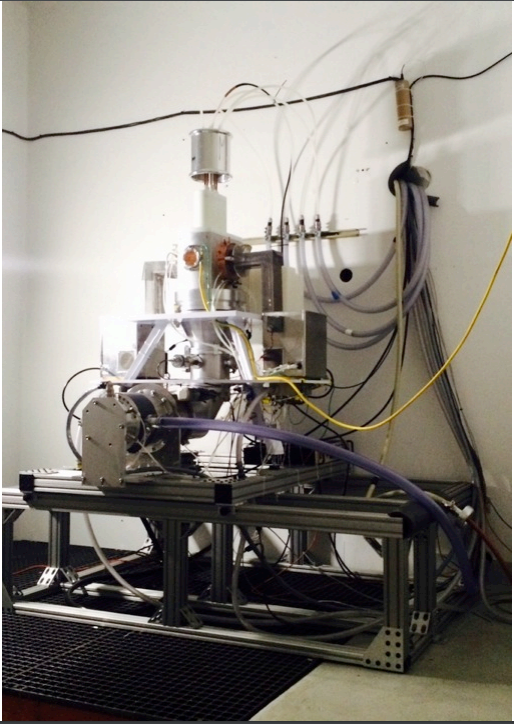
\includegraphics[width=\columnwidth]{./figures/Capture.PNG}
        \hspace{-5pt}\subfigimg[width=0.5\textwidth]{a)}{../nb_px_paper/figures/before_minimization_plot.pdf}{50}
%         \caption{ Decay curve for the isomeric transition of \ce{^{115m}In}.}
         %         \refstepcounter{subfigure}
         \label{fig:before_minimization}
   \hspace{-5pt}}%
     \subfloat{
        \centering

%         \subfigimg[width=0.5\textwidth]{b)}{./figures/after_minimization_plot.pdf}{50}
        \subfigimg[width=0.5\textwidth]{b)}{./figures/current_norm_az.pdf}{50}
         %         \refstepcounter{subfigure}
         \label{fig:after_minimization}
   \hspace{-5pt}}%
    \caption{\textred{Update this figure!!!} Results of variance minimization through enhancement of the effective areal density of the  aluminum degraders by \textred{2.52\%} (55\,MeV stack) and Kapton tape by \textred{2.52\%} (25\,MeV stack). A noticeable reduction of variance in measured proton fluence is seen,  particularly at the  rear stack positions.} 
%     Following minimization, additional apparent fluence is observed in the  \ce{^{nat}Al}(p,x)\ce{^{22}Na} and \ce{^{nat}Al}(p,x)\ce{^{24}Na} monitor channels, due to contamination from \ce{^{nat}Si}(p,x)\ce{^{22,24}Na} on the silicone adhesive used for sealing foil packets.}
     \label{fig:fe_variance_mins}
\end{figure}




An enhanced version of the final \ce{^{nat}Ti}(p,x)\ce{^{46}Sc}, \ce{^{nat}Ti}(p,x)\ce{^{48}V}, \ce{^{nat}Cu}(p,x)\ce{^{62}Zn}, and \ce{^{nat}Cu}(p,x)\ce{^{63}Zn} monitor reaction fluences is shown in \autoref{fig:fe_fluence_plot}.
% Without the reliable use of the  \ce{^{nat}Al}(p,x)\ce{^{22}Na} and \ce{^{nat}Al}(p,x)\ce{^{24}Na} monitor channels, local interpolation cannot be used for fluence assignment to the Nb foils, and global interpolation is reliant upon a validated model for fluence loss.
The uncertainty-weighted mean  for the two \ce{^{nat}Cu}(p,x) and two \ce{^{nat}Ti}(p,x) monitor channels was calculated at each energy position, to determine the final fluence assignments for the Cu and Ti foils, respectively, and the uncertainty-weighted mean  for all four monitor channels was used to determine the final fluence assignments for the Fe foils.
Uncertainty in proton fluence  is  calculated by error propagation of the fluence values  at each energy position.
These weighted-mean fluences are  plotted  in \autoref{fig:fe_fluence_plot}, along with the estimated fluence according to both  MCNP6 transport 
and an uncertainty-weighted linear $\chi^2$ fit to the individual monitor channel fluence measurements.
\textred{Both models reproduce the observed fluence data consistently within uncertainty, with the MCNP6 model predicting a slightly greater fluence loss throughout the stack.}
These models are used purely to provide an extrapolation from the highest-energy position back to the \enquote{front} of each stack, to compare with the nominal fluence measured by  the beamline current integrators.
% This involved minimizing on $\chi^2$ / degree of freedom, so that  a 95\% confidence interval in fluence would be reported as as well.
% As with the FWHM, a greater than 1$\sigma$ confidence interval is used for reporting fluence uncertainty to avoid an unrealistically small fluence confidence interval, based on the spread in observed fluence from Al and Cu monitor foils.
% The fluence and 2$\sigma$ uncertainties from this weighted-fit line are thus used in calculations of the various Nb(p,x) cross sections


% \begin{figure}
%  \centering
%  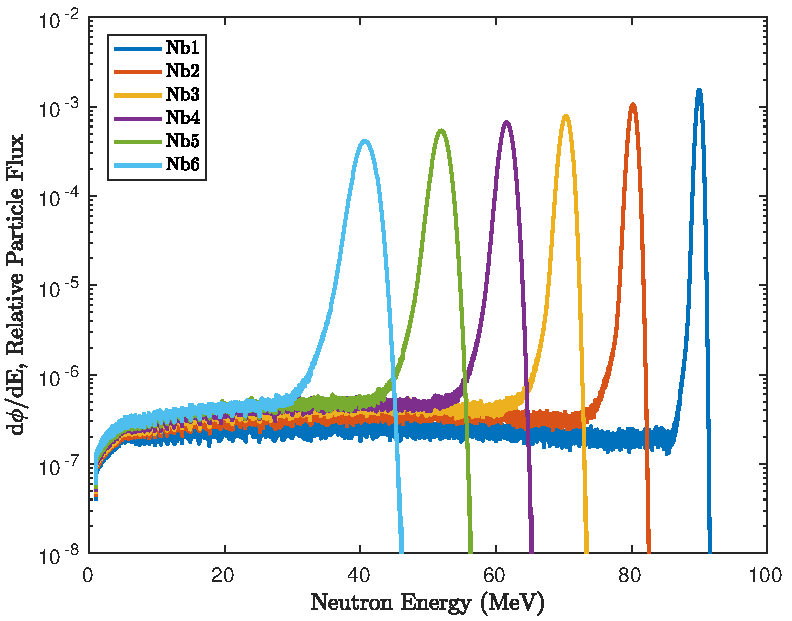
\includegraphics[width=0.5\linewidth]{./figures/Nb_ptallies.pdf}
%  % Nb_ptallies.pdf: 380x298 pixel, 72dpi, 13.41x10.51 cm, bb=0 0 380 298
%  \caption{Final variance minimized incident proton energy distributions for the Nb foils, as simulated in MCNP6. The distribution tallies in each foil are all normalized to be per source proton, which was $10^8$ in all simulations. As the beam is degraded, proton energy distributions become visibly broadened due to straggling, and drop in magnitude due to scattering losses.}
%  \label{fig:Nb_ptallies}
% \end{figure}

\begin{figure}
 \centering
%  \includegraphics[width=0.5\linewidth]{./figures/fe_fluence_plot.pdf}
 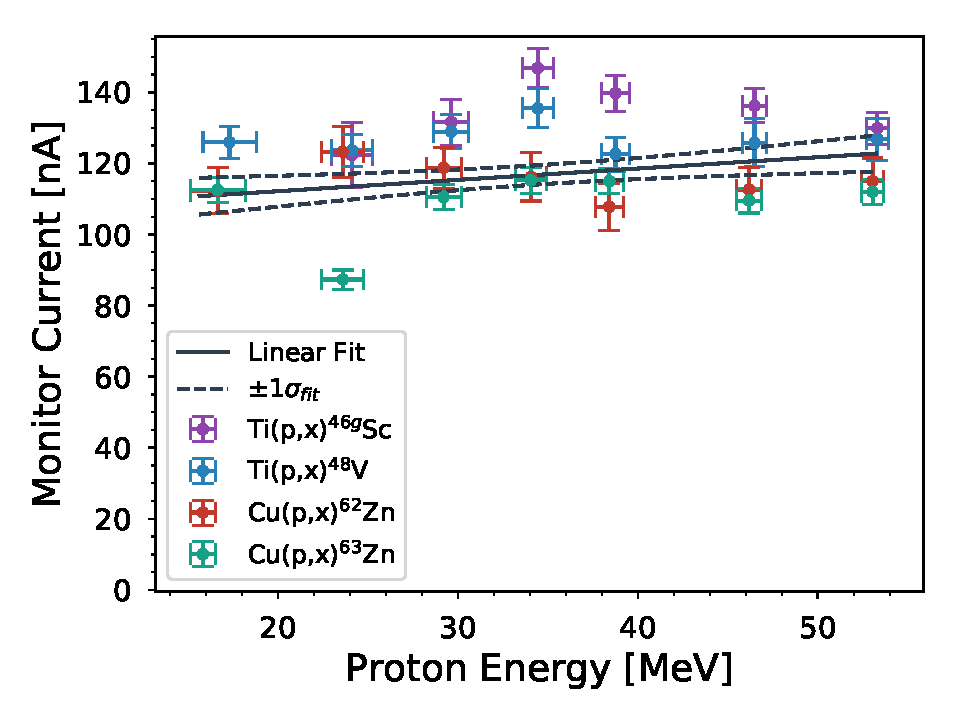
\includegraphics[width=0.5\linewidth]{./figures/current_norm_az.pdf}
 % Nb_ptallies.pdf: 380x298 pixel, 72dpi, 13.41x10.51 cm, bb=0 0 380 298
 \caption{\textred{Update this figure!!!} Final uncertainty-weighted mean proton fluences throughout the target stack, based on the variance-minimized observed fluence from the the  \ce{^{nat}Ti}(p,x)\ce{^{46}Sc}, \ce{^{nat}Ti}(p,x)\ce{^{48}V}, \ce{^{nat}Cu}(p,x)\ce{^{62}Zn}, and \ce{^{nat}Cu}(p,x)\ce{^{63}Zn} monitor reactions. 
%  A 95\% ($2\sigma$) confidence interval is reported in the fitted proton fluence, to ensure a realistic uncertainty in fluence, which encompasses the true absolute fluence. 
%   A clear loss of 
  The fluence  drops by approximately \textred{7.2--8.9\%} from the incident fluence of \textred{196.9--198.8 nAh} over the length of the target stack, based on fluence loss models from MCNP6 simulations and an empirical fit to  fluence measurements.}  
%   This is due to a combination of beam utilization, as well as scattering.}
 \label{fig:fe_fluence_plot}
\end{figure}






\subsection{\label{sec:calcs_sec_fe}Calculation of measured cross sections}


Using the quantified EoB activities along with the variance-minimized proton fluence, it is possible to calculate the final cross sections for the various observed (p,x) reactions.
While thin ($\approx$ 10--20\,mg/cm$^2$)  foils were irradiated to minimize the energy bins of these cross section measurements, it is important to note that all cross sections reported here are flux-averaged  
% cross sections, 
over the energy distribution subtended by each foil, as seen in \autoref{fig:Fe_ptallies}.
For both the cumulative and independent activities quantified, cross sections were calculated as:
\begin{equation}
\sigma = \dfrac{A_0 }{\rho \Delta r I \pp{1-e^{-\lambda \Delta t}} }
\end{equation}
where $A_0$ is the EoB activity for the monitor reaction product, $I$ is the proton current, $\rho \Delta r$ is the foil's areal density, $\lambda$ is the monitor reaction product's decay constant, and $\Delta t$ is the length of irradiation.
The beam current, measured using a current integrator connected to the electrically-isolated target box, remained stable for the duration of the irradiation.
The propagated uncertainty in cross section is calculated as the quadrature sum of the uncertainty in quantified EoB activity (which includes uncertainty in detector efficiencies), uncertainty in the duration of irradiation (conservatively estimated at 30\,s, to account for any minor transient changes in beam current), uncertainty in foil areal density, uncertainty in monitor product half-life (included, but normally negligible),  and uncertainty in proton current (quantified by error propagation of the monitor reaction fluence values  at each energy position, as seen in \autoref{fig:fe_fluence_plot}).


\begin{figure}
 \centering
 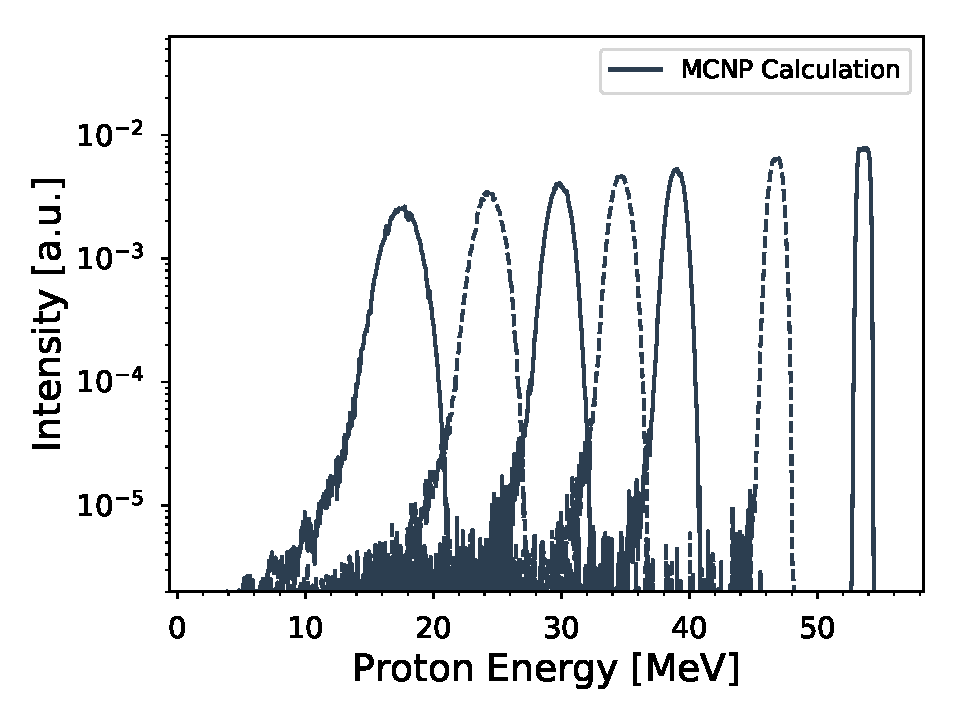
\includegraphics[width=0.5\linewidth]{./figures/Fe_mcnp_spectrum.pdf}
 % Nb_ptallies.pdf: 380x298 pixel, 72dpi, 13.41x10.51 cm, bb=0 0 380 298
 \caption{\textred{Add 25\,MeV stack tallies here! } Final variance minimized incident proton energy distributions for the Fe foils, as simulated in MCNP6. The distribution tallies in each foil are all normalized to be per source proton, which was $10^8$ in all simulations. As the beam is degraded, proton energy distributions become visibly broadened due to straggling, and drop in magnitude due to scattering losses.}
 \label{fig:Fe_ptallies}
\end{figure}


\section{\label{sec:results_fe}Results and Discussion}


\subsection{Measurement of nuclear excitation functions}

After irradiation, all foils were confirmed to still be sealed inside their Kapton packets, verifying that no activation products were lost due to packet failure and dispersal.
With the exception of two foils (Cu-20 and Ti-20), each activated foil had a small \enquote{blister} under the Kapton tape layer, caused by a combination of thermal swelling and the formation of short-lived beta activities.
% \comment{Maybe some Ne formed by Al(p,2a)Ne / Si(p,2ap)Ne?}
This blister   verifies that the primary proton beam was incident upon the foil, and provided the first evidence (before gamma-ray spectrometry) that the beam was stopped in the stack between Fe-14 and Ti-20.
Using the \ce{^{nat}Cu}(p,x)\ce{^{56}Co}, \ce{^{nat}Cu}(p,x)\ce{^{62}Zn}, and \ce{^{nat}Cu}(p,x)\ce{^{65}Zn} monitor reactions, as discussed in \autoref{sec:proton_transport_fe}, a fluence of \textred{198.8$\pm$6.7\,nAh} was calculated to be incident upon the 55\,MeV target stack using the MCNP6 fluence model, and a  fluence of \textred{196.9$\pm$11.3\,nAh} using the linear fit model.
Similarly, for the 25\,MeV stack, a fluence of \textred{198.8$\pm$6.7\,nAh} was calculated to be incident upon the 55\,MeV target stack using the MCNP6 fluence model, and a  fluence of \textred{196.9$\pm$11.3\,nAh} using the linear fit model.
\textred{All of these are consistent with the nominal fluence of 20.78\,nAh (for the 55\,MeV stack) and 31.61\,nAh (for the 25\,MeV stack) measured using the beamline current integrators.}
\textred{As fluence loss scales with $\sigma_{\mathrm{tot}}\rho\Delta r$, it is expected that an extrapolation back to the stack entrance (through the SS-3/SS-5 profile monitors) will underestimate the nominal fluence incident upon the box.}
This incident fluence dropped by approximately \textred{8.9\% to  180.9$\pm$5.4\,nAh (and by 7.2\% to  182.7$\pm$13.5\,nAh using the linear fit model)} over the length of the target stack, which is consistent with similar measurements at IPF in the past \cite{Voyles2018a,Graves2016}.
This loss of fluence is due to a combination of 
% beam utilization for the various 
(p,x) reactions throughout the target stack, as well as large-angle deflections (primarily in the aluminum degraders) from scattering of the beam.




Using the final proton fluence at each energy position, cross sections for  \textred{(list of residual products)} were extracted for (p,x) reactions  on \ce{^{nat}Fe} foils in the \textred{0--55\,MeV} region, as recorded in \autoref{tab:fe_rp_table}.
For  (p,x) reactions on \ce{^{nat}Cu} foils, the (p,x) cross sections for  \textred{(list of residual products)} were extracted, as recorded in \autoref{tab:cufe_rp_table}.
For  (p,x) reactions on \ce{^{nat}Ti} foils, the (p,x) cross sections for  \textred{(list of residual products)} were extracted, as recorded in \autoref{tab:ti_rp_table}.
In addition, as there exist a number of isomers with radioactive ground states in these mass regions,  independent measurements of isomer-to-ground-state branching ratios for \textred{\ce{^{52m/g}Mn},\ce{^{58m/g}Co},\ce{^{85m/g}Y},\ce{^{87m/g}Y}, and \ce{^{89m/g}Nb}} were  extracted and are recorded in \autoref{tab:fe_ibr_table}.
Comparisons  of the measured cross sections and isomer branching ratios with literature data (retrieved from EXFOR \cite{Otuka2014272}) are seen in the figures of Appendices \ref{sec:fe_xs_figures} and \ref{sec:fe_ibr_figures}.
The propagated uncertainty in these cross sections varies widely based on the reaction product in question, with the major components  arising from uncertainty in EoB activity \textred{($\pm$3--7\%), proton fluence ($\pm$4--6\%), and foil areal density ($\pm$0.1--0.6\%).}
% \comment{Update these with new numbers!\\ Stephen: Very impressive, if you feel this is realistic. }





% Please add the following required packages to your document preamble:
% \usepackage{booktabs}
\begin{table}
\centering
\caption{Measured cross sections for the various \ce{^{nat}Fe}(p,x) reaction products observed in this work. Cumulative cross sections are designated as $\sigma_c$, independent cross sections are designated as $\sigma_i$.}
\label{tab:fe_rp_table}
\small
% \resizebox{\textwidth}{!}{%
\begin{tabular}{@{}lllllll@{}}
\toprule
                            & \multicolumn{6}{c}{Production cross section (mb)}                                                                                                         \\ \cmidrule(l){2-7} 
E$_\text{p}$ (MeV)          & $89.74^{+0.48}_{-0.43}$ & $79.95^{+0.67}_{-0.64}$ & $70.17^{+0.91}_{-0.85}$ & $61.58^{+1.03}_{-0.98}$ & $52.10^{+1.25}_{-1.20}$ & $41.05^{+1.62}_{-1.54}$ \\ \midrule
% \ce{^{51}Cr}\,($\sigma_c$)  & $0.919\pm0.079$         & $0.373\pm0.023$         & $0.450\pm0.028$         & $0.303\pm0.016$         & --\cmmnt{\hrulefill}    & --\cmmnt{\hrulefill}    \\
% \ce{^{52}Mn}\,($\sigma_c$)  & $1.70\pm0.11$           & $0.570\pm0.031$         & $0.0407\pm0.0022$       & $0.00526\pm0.00057$     & --\cmmnt{\hrulefill}    & --\cmmnt{\hrulefill}    \\
% \ce{^{52g}Mn}\,($\sigma_i$) & $0.673\pm0.043$         & $0.239\pm0.018$         & $0.0164\pm0.0023$       & $0.000986\pm0.000053$   & --\cmmnt{\hrulefill}    & --\cmmnt{\hrulefill}    \\
% \ce{^{52m}Mn}\,($\sigma_c$) & $1.023\pm0.091$         & $0.331\pm0.030$         & $0.0244\pm0.0036$       & $0.00427\pm0.00052$     & --\cmmnt{\hrulefill}    & --\cmmnt{\hrulefill}    \\
% \ce{^{54}Mn}\,($\sigma_i$)  & $5.87\pm0.37$           & $3.77\pm0.21$           & $4.14\pm0.22$           & $4.84\pm0.26$           & $1.680\pm0.091$         & --\cmmnt{\hrulefill}    \\
% \ce{^{55}Co}\,($\sigma_c$)  & $1.71\pm0.11$           & $1.015\pm0.058$         & $0.193\pm0.012$         & $0.0299\pm0.0028$       & $0.00235\pm0.00022$     & --\cmmnt{\hrulefill}    \\
% \ce{^{56}Ni}\,($\sigma_c$)  & $0.0806\pm0.0051$       & $0.1005\pm0.0055$       & $0.0906\pm0.0046$       & $0.0304\pm0.0016$       & --\cmmnt{\hrulefill}    & --\cmmnt{\hrulefill}    \\
% \ce{^{57}Ni}\,($\sigma_c$)  & $1.465\pm0.093$         & $1.202\pm0.065$         & $1.400\pm0.071$         & $2.13\pm0.11$           & $1.565\pm0.083$         & $0.0262\pm0.0015$       \\
% \ce{^{57}Co}\,($\sigma_i$)  & $40.1\pm2.5$          & $35.6\pm1.9$          & $35.8\pm1.8$          & $48.5\pm2.5$            & $47.7\pm2.5$            & $3.21\pm0.18$           \\
% \ce{^{58}Co}\,($\sigma_c$)  & $57.7\pm4.5$            & $55.0\pm4.7$            & $42.7\pm3.4$            & $33.7\pm2.8$            & $39.0\pm3.8$            & $62.3\pm4.6$            \\
% \ce{^{58g}Co}\,($\sigma_i$) & $14.0\pm2.5$            & $10.8\pm2.1$            & $6.1\pm1.6$             & $7.8\pm1.4$             & $7.1\pm1.7$             & $1.12\pm0.32$           \\
% \ce{^{58m}Co}\,($\sigma_i$) & $43.6\pm3.7$            & $44.2\pm4.3$            & $36.6\pm3.0$            & $25.8\pm2.5$            & $31.9\pm3.3$            & $61.1\pm4.6$            \\
% \ce{^{59}Fe}\,($\sigma_c$)  & $0.865\pm0.057$         & $0.837\pm0.046$         & $0.749\pm0.039$         & $0.616\pm0.034$         & $0.209\pm0.014$         & --\cmmnt{\hrulefill}    \\
% \ce{^{60}Co}\,($\sigma_c$)  & $13.23\pm0.87$          & $13.47\pm0.78$          & $11.14\pm0.94$          & $11.44\pm0.80$          & $9.30\pm0.87$           & $6.6\pm1.1$             \\
% \ce{^{61}Cu}\,($\sigma_c$)  & $50.5\pm3.3$            & $56.1\pm3.2$            & $65.1\pm3.6$            & $72.2\pm4.0$            & $80.6\pm4.7$            & $157.1\pm8.6$           \\
\ce{^{64}Cu}\,($\sigma_i$)  & $38.7\pm2.7$            & $42.8\pm2.4$            & $45.5\pm2.7$            & $50.2\pm2.8$            & $55.7\pm3.0$            & $63.3\pm3.6$                 \\ \bottomrule
\end{tabular}
% }
\end{table}

% Please add the following required packages to your document preamble:
% \usepackage{booktabs}
\begin{table}
\centering
\caption{Measured cross sections for the various \ce{^{nat}Cu}(p,x) reaction products observed in this work. Cumulative cross sections are designated as $\sigma_c$, independent cross sections are designated as $\sigma_i$.}
\label{tab:cufe_rp_table}
\small
% \resizebox{\textwidth}{!}{%
\begin{tabular}{@{}lllllll@{}}
\toprule
                            & \multicolumn{6}{c}{Production cross section (mb)}                                                                                                         \\ \cmidrule(l){2-7} 
E$_\text{p}$ (MeV)          & $89.74^{+0.48}_{-0.43}$ & $79.95^{+0.67}_{-0.64}$ & $70.17^{+0.91}_{-0.85}$ & $61.58^{+1.03}_{-0.98}$ & $52.10^{+1.25}_{-1.20}$ & $41.05^{+1.62}_{-1.54}$ \\ \midrule
% \ce{^{51}Cr}\,($\sigma_c$)  & $0.919\pm0.079$         & $0.373\pm0.023$         & $0.450\pm0.028$         & $0.303\pm0.016$         & --\cmmnt{\hrulefill}    & --\cmmnt{\hrulefill}    \\
% \ce{^{52}Mn}\,($\sigma_c$)  & $1.70\pm0.11$           & $0.570\pm0.031$         & $0.0407\pm0.0022$       & $0.00526\pm0.00057$     & --\cmmnt{\hrulefill}    & --\cmmnt{\hrulefill}    \\
% \ce{^{52g}Mn}\,($\sigma_i$) & $0.673\pm0.043$         & $0.239\pm0.018$         & $0.0164\pm0.0023$       & $0.000986\pm0.000053$   & --\cmmnt{\hrulefill}    & --\cmmnt{\hrulefill}    \\
% \ce{^{52m}Mn}\,($\sigma_c$) & $1.023\pm0.091$         & $0.331\pm0.030$         & $0.0244\pm0.0036$       & $0.00427\pm0.00052$     & --\cmmnt{\hrulefill}    & --\cmmnt{\hrulefill}    \\
% \ce{^{54}Mn}\,($\sigma_i$)  & $5.87\pm0.37$           & $3.77\pm0.21$           & $4.14\pm0.22$           & $4.84\pm0.26$           & $1.680\pm0.091$         & --\cmmnt{\hrulefill}    \\
% \ce{^{55}Co}\,($\sigma_c$)  & $1.71\pm0.11$           & $1.015\pm0.058$         & $0.193\pm0.012$         & $0.0299\pm0.0028$       & $0.00235\pm0.00022$     & --\cmmnt{\hrulefill}    \\
% \ce{^{56}Ni}\,($\sigma_c$)  & $0.0806\pm0.0051$       & $0.1005\pm0.0055$       & $0.0906\pm0.0046$       & $0.0304\pm0.0016$       & --\cmmnt{\hrulefill}    & --\cmmnt{\hrulefill}    \\
% \ce{^{57}Ni}\,($\sigma_c$)  & $1.465\pm0.093$         & $1.202\pm0.065$         & $1.400\pm0.071$         & $2.13\pm0.11$           & $1.565\pm0.083$         & $0.0262\pm0.0015$       \\
% \ce{^{57}Co}\,($\sigma_i$)  & $40.1\pm2.5$          & $35.6\pm1.9$          & $35.8\pm1.8$          & $48.5\pm2.5$            & $47.7\pm2.5$            & $3.21\pm0.18$           \\
% \ce{^{58}Co}\,($\sigma_c$)  & $57.7\pm4.5$            & $55.0\pm4.7$            & $42.7\pm3.4$            & $33.7\pm2.8$            & $39.0\pm3.8$            & $62.3\pm4.6$            \\
% \ce{^{58g}Co}\,($\sigma_i$) & $14.0\pm2.5$            & $10.8\pm2.1$            & $6.1\pm1.6$             & $7.8\pm1.4$             & $7.1\pm1.7$             & $1.12\pm0.32$           \\
% \ce{^{58m}Co}\,($\sigma_i$) & $43.6\pm3.7$            & $44.2\pm4.3$            & $36.6\pm3.0$            & $25.8\pm2.5$            & $31.9\pm3.3$            & $61.1\pm4.6$            \\
% \ce{^{59}Fe}\,($\sigma_c$)  & $0.865\pm0.057$         & $0.837\pm0.046$         & $0.749\pm0.039$         & $0.616\pm0.034$         & $0.209\pm0.014$         & --\cmmnt{\hrulefill}    \\
% \ce{^{60}Co}\,($\sigma_c$)  & $13.23\pm0.87$          & $13.47\pm0.78$          & $11.14\pm0.94$          & $11.44\pm0.80$          & $9.30\pm0.87$           & $6.6\pm1.1$             \\
% \ce{^{61}Cu}\,($\sigma_c$)  & $50.5\pm3.3$            & $56.1\pm3.2$            & $65.1\pm3.6$            & $72.2\pm4.0$            & $80.6\pm4.7$            & $157.1\pm8.6$           \\
\ce{^{64}Cu}\,($\sigma_i$)  & $38.7\pm2.7$            & $42.8\pm2.4$            & $45.5\pm2.7$            & $50.2\pm2.8$            & $55.7\pm3.0$            & $63.3\pm3.6$                 \\ \bottomrule
\end{tabular}
% }
\end{table}

% Please add the following required packages to your document preamble:
% \usepackage{booktabs}
\begin{table}
\centering
\caption{Measured cross sections for the various \ce{^{nat}Ti}(p,x) reaction products observed in this work. Cumulative cross sections are designated as $\sigma_c$, independent cross sections are designated as $\sigma_i$.}
\label{tab:ti_rp_table}
\small
% Disable next line for journal submission
% \resizebox{\textwidth}{!}{%
\begin{tabular}{@{}lllllll@{}}
\toprule
                            & \multicolumn{6}{c}{Production cross section (mb)}                                                                                                         \\ \cmidrule(l){2-7} 
E$_\text{p}$ (MeV)          & $89.37^{+0.47}_{-0.45}$ & $79.55^{+0.68}_{-0.64}$ & $69.70^{+0.90}_{-0.85}$ & $61.07^{+1.05}_{-0.98}$ & $51.51^{+1.25}_{-1.21}$ & $40.34^{+1.58}_{-1.55}$ \\ \midrule
% \ce{^{82m}Rb}\,($\sigma_c$) & $2.48\pm0.22$           & --\cmmnt{\hrulefill}    & --\cmmnt{\hrulefill}    & --\cmmnt{\hrulefill}    & --\cmmnt{\hrulefill}    & --\cmmnt{\hrulefill}    \\
% \ce{^{83}Sr}\,($\sigma_c$)  & $4.02\pm0.61$           & $4.78\pm0.42$           & $3.49\pm0.36$           & --\cmmnt{\hrulefill}    & --\cmmnt{\hrulefill}    & --\cmmnt{\hrulefill}    \\
% \ce{^{85}Y}\,($\sigma_c$)   & $13.78\pm0.55$          & $7.52\pm0.51$           & $2.11\pm0.14$           & --\cmmnt{\hrulefill}    & --\cmmnt{\hrulefill}    & --\cmmnt{\hrulefill}    \\
% \ce{^{85g}Y}\,($\sigma_i$)  & $2.37\pm0.11$           & $2.08\pm0.17$           & $0.557\pm0.037$         & --\cmmnt{\hrulefill}    & --\cmmnt{\hrulefill}    & --\cmmnt{\hrulefill}    \\
% \ce{^{85m}Y}\,($\sigma_i$)  & $11.41\pm0.54$          & $5.44\pm0.48$           & $1.55\pm0.13$           & --\cmmnt{\hrulefill}    & --\cmmnt{\hrulefill}    & --\cmmnt{\hrulefill}    \\
% \ce{^{86}Zr}\,($\sigma_c$)  & $12.68\pm0.68$          & $18.21\pm0.93$          & $19.28\pm0.97$          & $6.16\pm0.32$           & --\cmmnt{\hrulefill}    & --\cmmnt{\hrulefill}    \\
% \ce{^{86}Y}\,($\sigma_i$)   & $33.4\pm1.8$            & $41.6\pm2.2$            & $39.9\pm2.1$            & $13.56\pm0.72$          & --\cmmnt{\hrulefill}    & --\cmmnt{\hrulefill}    \\
% \ce{^{87}Zr}\,($\sigma_c$)  & $47.4\pm7.3$            & $28.0\pm2.8$            & $32.2\pm2.9$            & $49.8\pm5.0$            & $38.2\pm3.7$            & $1.12\pm0.17$           \\
% \ce{^{87}Y}\,($\sigma_i$)   & $110.0\pm7.2$           & $54.7\pm2.8$            & $61.0\pm2.9$            & $90.0\pm4.9$            & $67.2\pm3.6$            & $2.91\pm0.17$           \\
% \ce{^{87g}Y}\,($\sigma_i$)  & $28.0\pm5.8$            & $7.4\pm1.3$             & $6.55\pm0.64$           & $5.8\pm2.2$             & $2.63\pm0.47$           & $0.942\pm0.073$         \\
% \ce{^{87m}Y}\,($\sigma_i$)  & $82.0\pm4.3$            & $47.3\pm2.5$            & $54.4\pm2.8$            & $84.2\pm4.4$            & $64.6\pm3.6$            & $1.97\pm0.15$           \\
% \ce{^{88}Zr}\,($\sigma_c$)  & $159.1\pm7.8$           & $144.6\pm6.8$           & $62.4\pm3.1$            & $21.2\pm1.0$            & $33.6\pm1.8$            & $65.3\pm4.0$            \\
% \ce{^{88}Y}\,($\sigma_i$)   & $17.2\pm1.1$            & $13.27\pm0.86$          & $7.98\pm0.72$           & $2.91\pm0.25$           & $9.2\pm1.4$             & $9.88\pm0.69$           \\
% \ce{^{89}Nb}\,($\sigma_c$)  & --\cmmnt{\hrulefill}    & --\cmmnt{\hrulefill}    & $179\pm14$              & $214.4\pm9.8$           & --\cmmnt{\hrulefill}    & --\cmmnt{\hrulefill}    \\
% \ce{^{89g}Nb}\,($\sigma_i$) & --\cmmnt{\hrulefill}    & --\cmmnt{\hrulefill}    & $145\pm14$              & $186.4\pm9.6$           & --\cmmnt{\hrulefill}    & --\cmmnt{\hrulefill}    \\
% \ce{^{89m}Nb}\,($\sigma_i$) & --\cmmnt{\hrulefill}    & --\cmmnt{\hrulefill}    & $34.7\pm2.6$            & $28.0\pm2.0$            & --\cmmnt{\hrulefill}    & --\cmmnt{\hrulefill}    \\
% \ce{^{89}Zr}\,($\sigma_i$)  & $211\pm11$              & $243\pm13$              & $294\pm15$              & $257\pm13$              & $55.4\pm3.0$            & $15.5\pm1.0$            \\
% \ce{^{90}Mo}\,($\sigma_i$)  & $21.3\pm1.1$            & $26.4\pm1.3$            & $34.5\pm1.6$            & $61.9\pm3.1$            & $122.0\pm6.1$           & $24.2\pm1.5$            \\
% \ce{^{90}Nb}\,($\sigma_i$)  & $158.3\pm8.1$           & $174.9\pm8.5$           & $209.3\pm9.9$           & $272\pm14$              & $369\pm19$              & $163.9\pm9.8$           \\
% \ce{^{91m}Nb}\,($\sigma_c$) & --\cmmnt{\hrulefill}    & --\cmmnt{\hrulefill}    & --\cmmnt{\hrulefill}    & --\cmmnt{\hrulefill}    & --\cmmnt{\hrulefill}    & $66.5\pm5.8$            \\
% \ce{^{92m}Nb}\,($\sigma_i$) & $43.7\pm2.4$            & $47.3\pm2.4$            & $49.8\pm2.6$            & $52.9\pm2.8$            & $55.3\pm3.1$            & $59.9\pm3.9$            \\
\ce{^{93m}Mo}\,($\sigma_i$) & $0.97\pm0.20$           & $1.29\pm0.15$           & $1.62\pm0.24$           & $1.85\pm0.15$           & $1.86\pm0.14$           & $2.00\pm0.15$               \\ \bottomrule
\end{tabular}
% }
\end{table}






% Please add the following required packages to your document preamble:
% \usepackage{booktabs}
\begin{table}
\centering
\caption{Measured isomer-to-ground-state branching ratios for the various \ce{^{nat}Fe}(p,x), \ce{^{nat}Cu}(p,x), and \ce{^{nat}Ti}(p,x) reaction products observed in this work.}
\label{tab:fe_ibr_table}
\small
% \resizebox{\textwidth}{!}{%
\begin{tabular}{@{}lllllll@{}}
\toprule
                               & \multicolumn{6}{c}{Isomer branching ratio}                                                                                                                \\ \cmidrule(l){2-7} 
E$_\text{p}$ (MeV)             & $89.74^{+0.48}_{-0.43}$ & $79.95^{+0.67}_{-0.64}$ & $70.17^{+0.91}_{-0.85}$ & $61.58^{+1.03}_{-0.98}$ & $52.10^{+1.25}_{-1.20}$ & $41.05^{+1.62}_{-1.54}$ \\ \midrule
\ce{^{nat}Cu}(p,x)\ce{^{52}Mn} & $0.603\pm0.066$         & $0.581\pm0.062$         & $0.598\pm0.095$         & $0.81\pm0.13$           & --\cmmnt{\hrulefill}    & --\cmmnt{\hrulefill}    \\
\ce{^{nat}Cu}(p,x)\ce{^{58}Co} & $0.757\pm0.088$         & $0.80\pm0.10$         & $0.858\pm0.099$         & $0.767\pm0.097$         & $0.82\pm0.12$           & $0.98\pm0.10$            \vspace{1em}     \\ 
E$_\text{p}$ (MeV)             & $89.37^{+0.47}_{-0.45}$ & $79.55^{+0.68}_{-0.64}$ & $69.70^{+0.90}_{-0.85}$ & $61.07^{+1.05}_{-0.98}$ & $51.51^{+1.25}_{-1.21}$ & $40.34^{+1.58}_{-1.55}$ \\ \midrule
\ce{^{nat}Nb}(p,x)\ce{^{85}Y}  & $0.828\pm0.051$         & $0.724\pm0.080$         & $0.736\pm0.080$         & --\cmmnt{\hrulefill}    & --\cmmnt{\hrulefill}    & --\cmmnt{\hrulefill}    \\
\ce{^{nat}Nb}(p,x)\ce{^{87}Y}  & $0.746\pm0.063$         & $0.865\pm0.063$         & $0.893\pm0.063$         & $0.936\pm0.070$         & $0.961\pm0.075$         & $0.676\pm0.065$         \\
\ce{^{nat}Nb}(p,x)\ce{^{89}Nb} & --\cmmnt{\hrulefill}    & --\cmmnt{\hrulefill}    & $0.193\pm0.021$         & $0.130\pm0.011$         & --\cmmnt{\hrulefill}    & --\cmmnt{\hrulefill}    \\ \bottomrule
\end{tabular}
% }
\end{table}



\textred{Placeholder text follows...fill in actual discussion of results...}

% lee:
% 
% In addition to the interest in the production of 51,52 Mn for PET research, this experiment offered
% an opportunity to study the distribution of angular momentum in compound nuclear and direct
% pre-equilibrium reactions via observation of the 52g Mn (t ½ =5.591±0.003 d; J π =6 + ) to 52m Mn
% (t ½ =21.1±0.2 m; J π =2 + ) ratio. These results indicated were presented at the University of Oslo in
% May 2017 5 and indicate that the constant
% temperature nuclear level density model
% which has had the greatest success at
% reproducing most low-energy nuclear
% reaction data fails to reproduce the
% deposition of angular momentum at both
% compound and pre-compound energies
% (see figure 3). This result will be
% discussed in greater detail in Mr. Andrew
% Voyles’ doctoral dissertation, which is
% expected to be completed by May 2018.



These results have several notable features.
The various \ce{^{nat}Cu}(p,x) cross sections measured here are in excellent agreement with the body of measurements in the literature,  but have been measured nearly exclusively with the highest precision to date.
Similarly, the various \ce{^{nat}Nb}(p,x) cross sections measured here are in excellent agreement with literature data, which is far more sparse in the 40--90\,MeV region than for \ce{^{nat}Cu}(p,x) ---  fewer than three existing measurements have been performed for the majority of the reactions presented here.
Indeed,  the \ce{^{nat}Nb}(p,x)\ce{^{83}Sr}, \ce{^{nat}Nb}(p,x)\ce{^{85}Y}, \ce{^{nat}Nb}(p,x)\ce{^{89}Nb}, \ce{^{nat}Nb}(p,x)\ce{^{90}Mo}, \ce{^{nat}Nb}(p,x)\ce{^{91m}Nb}, and \ce{^{nat}Nb}(p,x)\ce{^{98m}Mo} reactions each possess no more than a total of three data points in this energy region.
Not only do the \ce{^{nat}Nb}(p,x) measurements in this work fill in the sparse data in this energy region, but they have been measured with the highest precision relative to existing literature data.



% Furthermore, t
This work presents the first measurements of several observables in 
% these mass regions.
% This work reports the first experimental measurement of
this mass region, including the \ce{^{nat}Nb}(p,x)\ce{^{82m}Rb} reaction in the 40--90\,MeV region, 
% It also represents  the first measurement of 
the independent cross section for       \ce{^{nat}Cu}(p,x)\ce{^{52\text{g}}Mn}, and the \ce{^{52\text{m}}Mn} ($2^+$) / \ce{^{52\text{g}}Mn}  ($6^+$)  isomer branching ratio via \ce{^{nat}Cu}(p,x).  
The cumulative cross sections from these data are also consistent with existing measurements of the cumulative \ce{^{nat}Cu}(p,x)\ce{^{52}Mn} cross section.
Similarly, this work offers the first measurement of the independent cross sections for \ce{^{nat}Nb}(p,x)\ce{^{85\text{g}}Y},  as well as the first measurement of the     \ce{^{85\text{m}}Y} (\nicefrac{9}{2}$^+$) / \ce{^{85\text{g}}Y}   (\nicefrac{1}{2}$^-$)
% (${^{1}/_{2}}^{-}$)
% ($\sfrac{1}{2}^-$) 
isomer branching ratio via \ce{^{nat}Nb}(p,x).


\textred{Comment on details of 51/52Mn production here...}


Notably, this work is the most well-characterized measurement of the \ce{^{nat}Nb}(p,x)\ce{^{90}Mo} reaction below 100\,MeV to date, with cross sections measured  at the 4--6\% uncertainty level.
This is important, as it presents the first step towards characterizing this reaction for use as a proton monitor reaction standard below 100\,MeV.
% The quantification of \ce{^{90}Mo} activity proved to be one of the most straightforward of all reaction products observed in this work.
\ce{^{nat}Nb}(p,x)\ce{^{90}Mo} can only be populated through the (p,4n) reaction channel, so no corrections for (n,x) contamination channels or decay down the A=90 isobar are needed.
% , which makes activity quantification trivial.
% In addition, 
\ce{^{90}Mo}  possesses seven strong, distinct gamma lines which can easily  be used for its identification and quantification.
Finally, the production of \ce{^{90}Mo}  in the 40--90\,MeV region is quite strong, with a peak cross section of approximately 120 mb.
Combining the reaction yield and gamma abundance, the use of approximately 23\,mg/cm$^2$ Nb targets easily provided sufficient counting statistics for activity quantification in the 40--90\,MeV region.
This result presents the first step towards the use of \ce{^{90}Mo} as a clean and precise   charged particle monitor reaction standard in irradiations up to approximately 24\,h in duration.



\textred{Placeholder text follows...Comment on production pathways of medical radionuclides...}



In addition to the $^\text{nat}$Nb(p,x)\ce{^{90}Mo} measurement, this experiment has also yielded measurements of  a number of additional  emerging radionuclides with medical applications.
These include the non-standard positron emitters 
\ce{^{57}Ni} \cite{PMID:7632762,zweit1996medium,Graves2016,Rosch2014}, 
\ce{^{64}Cu} \cite{Lewis2003,Bandari2014,mp500671j,Szelecsenyi1993,Aslam2009,Hilgers2003,Szelecsenyi2005,Voyles2017},  \ce{^{86}Y} \cite{Valdovinos2017,Nickles2003,Qaim2008,QaimSyedM2011,Rosch1993,doi:10.1139/v67-193,levkovski1991cross,Johnson2015,Singh2013,Kiselev1974,Kandil2009}, 
\ce{^{89}Zr}  \cite{Verel2003,Dijkers2009,Dijkers2010,PhysRevC.38.1624,Omara2009},  
\ce{^{90}Nb} \cite{Busse2002,Radchenko2012},  
% the $\beta^-$-therapy agent  \ce{^{64}Cu},  
and the Auger-therapy agent \ce{^{82\text{m}}Rb} \cite{Kovacs1991,Titarenko2011}. 
Production of these radionuclides offers no major advantages over established pathways, with the generally lower yields and radioisotopic purities failing to justify the convenience of natural targets  via   \ce{^{nat}Cu}(p,x) and  \ce{^{nat}Nb}(p,x). 
The one possible exception to this trend is the non-standard positron emitter \ce{^{57}Ni} ($t_{1/2}=35.60\pm0.06$ h, $\epsilon$=100\% to \ce{^{57}Co} \cite{Bhat1998}) --- the \ce{^{57}Ni}/\ce{^{56}Ni} ratio of production rates is approximately 290 at 61.58\,MeV, and varies from 45--75 at the 70--90\,MeV positions.
This \ce{^{nat}Cu}(p,x) route offers both higher yield and higher radioisotopic purity over the established  \ce{^{nat}Co}(p,3n) pathway, which suffers from approximately fivefold greater  \ce{^{56}Ni} contamination \cite{MICHEL1997153,Ditrói2013}.




\subsection{Comparison of reaction modeling with experimental results}



% In this work
As mentioned before, cumulative cross sections are reported here for the first observable product nuclei in a mass chain, or whenever it is impossible to use decay spectrometry to distinguish direct production of a nucleus from decay feeding.
For all remaining observed reaction products in the mass chain, and cases where no decay precursors exist, independent cross sections are reported, allowing for determination of the direct production via subtraction.  
This, in turn, offers the opportunity to 
% use these data to gain insight into 
gauge the predictive capabilities of modern nuclear models used in the reaction evaluation process.  
The reaction channels with independent cross sections were compared to calculations with the reaction modeling codes EMPIRE, TALYS, and CoH, run with the default settings. 
The default optical models and E1 gamma strength function models for each code are presented in Table \ref{tab:defaults}. 
The large energy range covered by many of the exit channels, which extends significantly beyond the range of pure compound nuclear/evaporation, allows the data to be used to study the differences between these modeling codes in the  pre-equilibrium regime.
% All three codes use a two-exciton phenomenological model to calculate the pre-equilibrium cross section, but the specific implementation differs between the codes. 


The default level density in both CoH and TALYS is the Gilbert-Cameron model, which uses a Constant Temperature model below a critical energy and Fermi Gas model above it.
% \cite{add_level_density_models_here}. 
The default level density in EMPIRE is the Enhanced Generalized Superfluid Model (EGSM) which uses the Generalized Superfluid model below a critical energy, and Fermi Gas model above it \cite{Capote2009}.
% \cite{add_level_density_models_here}.
The EGSM densities are normalized to $D_0$ and the discrete levels, but in such a way that only the level density below the neutron separation energy is  effected by the discrete levels chosen for the normalization.  
All three codes use a two-exciton phenomenological model to calculate the pre-equilibrium cross section, but the specific implementation differs between the codes. 


% \def\arraystretch{1.5}
\begin{table}
 \caption{Default settings for the reactions codes}
 \label{tab:defaults}
 \resizebox{\textwidth}{!}{%
\begin{tabular}{ c c c c}

 \underline{Code Version} & \underline{Proton/Neutron Optical Model} & \underline{Alpha Optical Model}  & \underline{E1 $\gamma$SF Model}  \\ 
 EMPIRE-3.2.3\cite{Herman2007}       & Koning-Delaroche\cite{Koning2003} & Avrigeanu(2009)\cite{Avrigeanu2009}       & Modified Lorentzian\cite{belgya2006handbook}  \\  
 TALYS-1.8\cite{Koning2012}          & Koning-Delaroche & Specific folded potential\cite{Koning2012}      & Brink-Axel Lorentzian\cite{Koning2012}   \\
  CoH-3.5.1\cite{kawano2003coh,KAWANO2010} & Koning-Delaroche     & Avrigeanu(1994)\cite{Avrigeanu1994} & Generalized Lorentzian\cite{kawano2003coh,KAWANO2010}
  
\end{tabular}
}
\end{table}

% The modeling of several of the \ce{^{93}Nb} residual production cross sections are studied in detail here. 
% Only total channel residual 
Given the large number of exit channels in this data set, we will limit our discussion to  cross sections for the production of a specific residual nucleus with experimental data through the full rise and fall of the peak, 
% that have only one reaction channel, and that are 
and at least 1\% of the total reaction cross section.
% are discussed in detail. 
% Residual production
Exit channel cross sections that do not exhibit the full rise and fall of the peak, which is identified as 
% the compound portion of the cross section
being dominated by the formation of a compound nucleus, do not provide enough information to analyze the calculations.
% Some residuals, such as 
Residual nuclei like \ce{^{88}Zr} that can be produced by multiple reaction channels, such as (p,$\alpha$2n) and by (p,2p4n)  are also not discussed in depth. 
% Both compound peaks are seen in the data and cannot be separated, so such residuals are not included in the detailed analysis.
% Very small channels, 
We exclude reactions with cross sections with peak values less than 1\% of the total reaction cross section 
% are excluded because the modeling of their cross sections is 
because their behavior is extremely sensitive  to  more dominant  channels.
The three residual nuclei that meet all of the above criteria for which there is an independent measurement of the residual production cross section are \ce{^{86}Y}, \ce{^{90}Mo}, and \ce{^{90}Nb}.


The \ce{^{93}Nb}(p,$\alpha$p3n)\ce{^{86}Y} reaction channel, which peaks at approximately \mbox{70\,MeV}, is well within the compound regime for the entire energy region of this experiment (\autoref{fig:86Y}).
The data collected on this residual is consistent with the one other data set available, taken in 1997 by Michel \emph{et al.} \cite{MICHEL1997153}. 
The \ce{^{93}Nb}(p,4n)\ce{^{90}Mo} and \ce{^{93}Nb}(p,p3n)\ce{^{90}Nb} channels both peak early in the energy region, around 50\,MeV, and the data clearly show the full rise, peak, and fall of the compound cross section (\autoref{fig:90Mo} \& \ref{fig:90Nb}). 
In both of these channels, this data  is consistent with the data by Titarenko \emph{et al.} in 2011 \cite{Titarenko2011}.

The \ce{^{90}Nb} production cross section exhibits a persistent pre-equilibrium \enquote{tail} that keeps the channel open  well after the compound cross section has fallen away. 
TALYS, TENDL, and CoH seem to have the correct shape for this pre-equilibrium cross section, with magnitudes that are just slightly too low.
EMPIRE, however, does not level off  as much as the data and the other codes are seen to, and misses the high-energy data points.

\begin{figure}
 \centering
 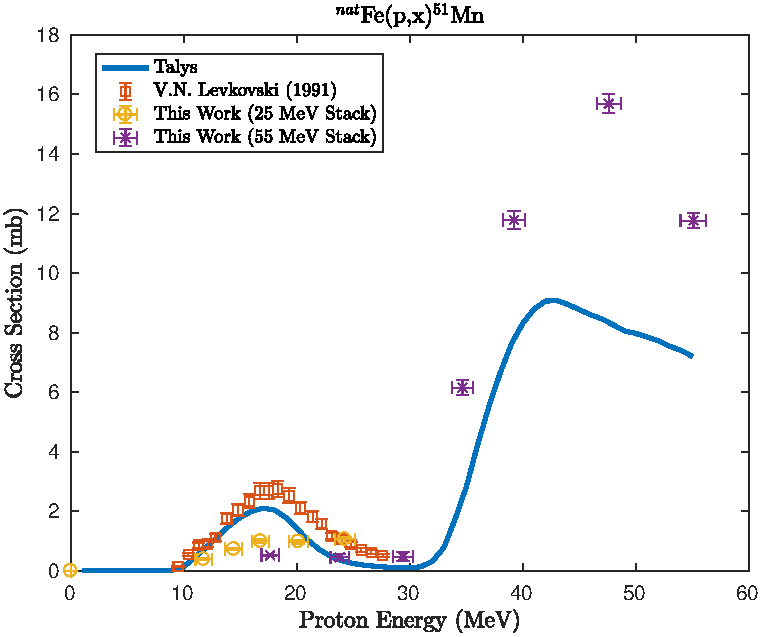
\includegraphics[width=0.5\linewidth]{./figures/51Mn_px.pdf}
 % Nb_ptallies.pdf: 380x298 pixel, 72dpi, 13.41x10.51 cm, bb=0 0 380 298
 \caption{Measured \ce{^{93}Nb}(p,x)\ce{^{86}Y} cross section, with the \ce{^{93}Nb}(p,$\alpha$p3n)\ce{^{86}Y} reaction channel visibly peaking at approximately \mbox{70 MeV}.}
 \label{fig:86Y}
\end{figure}




\begin{figure}
 \centering
 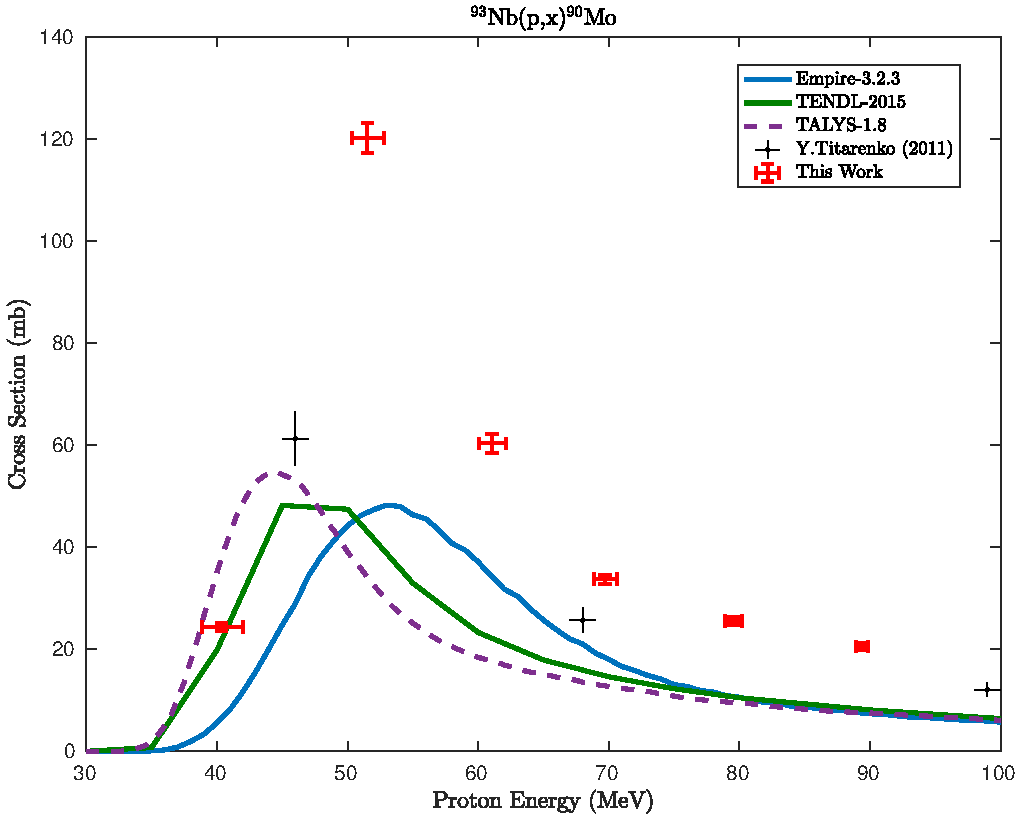
\includegraphics[width=0.5\linewidth]{../nb_px_paper/figures/90Mo.pdf}
 % Nb_ptallies.pdf: 380x298 pixel, 72dpi, 13.41x10.51 cm, bb=0 0 380 298
 \caption{Measured \ce{^{93}Nb}(p,x)\ce{^{90}Mo} cross section, with the \ce{^{93}Nb}(p,4n)\ce{^{90}Mo} reaction channel visibly peaking at approximately \mbox{50 MeV}.}
 \label{fig:90Mo}
\end{figure}


\begin{figure}
 \centering
 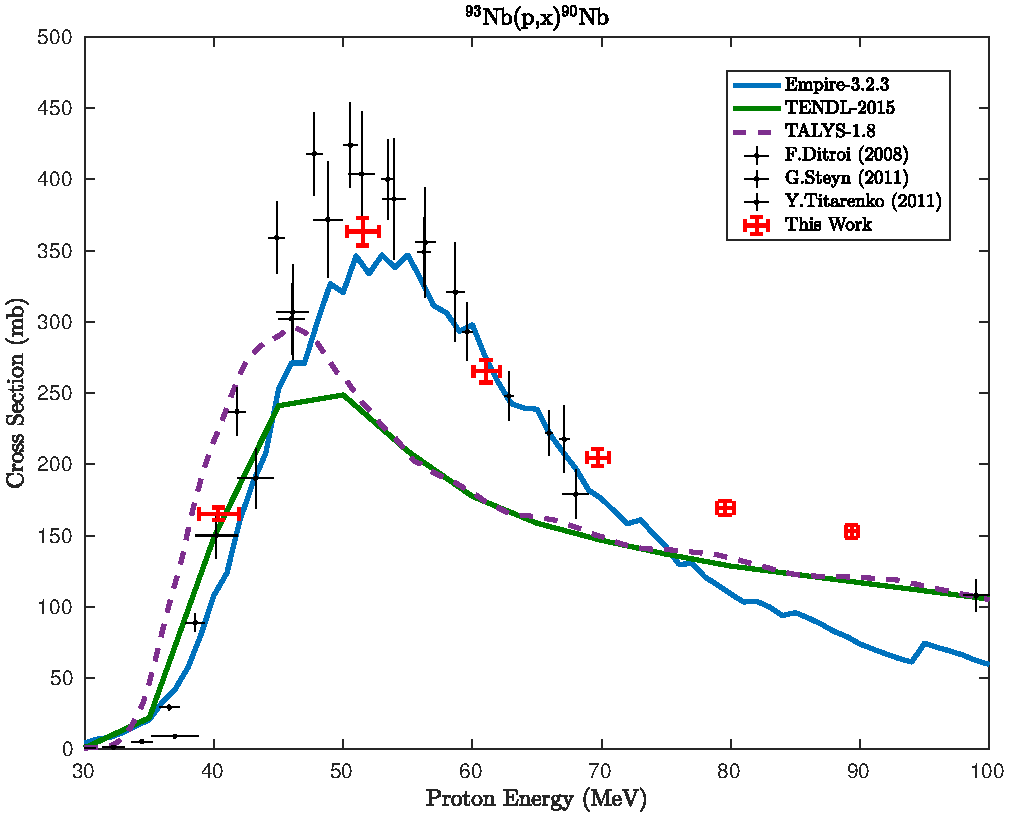
\includegraphics[width=0.5\linewidth]{../nb_px_paper/figures/90Nb.pdf}
 % Nb_ptallies.pdf: 380x298 pixel, 72dpi, 13.41x10.51 cm, bb=0 0 380 298
 \caption{Measured \ce{^{93}Nb}(p,x)\ce{^{90}Nb} cross section, with the \ce{^{93}Nb}(p,p3n)\ce{^{90}Nb} reaction channel visibly peaking at approximately \mbox{50 MeV}.}
 \label{fig:90Nb}
\end{figure}




In all three channels, the TALYS, TENDL, and CoH calculations rise, peak, and fall at lower energies than the data, while EMPIRE calculates the peak to occur at higher energies.
For \ce{^{90}Mo}, the EMPIRE peak is representative of the data.
For \ce{^{86}Y} and \ce{^{90}Nb}, the peak is missed by all three  of the codes.


The magnitudes of the TALYS and TENDL calculations are consistently too low in the three channels studied here. 
For \ce{^{86}Y}, CoH and EMPIRE also predict smaller cross sections than the data would suggest, which may be influenced by incorrect modeling of other, stronger, channels.
The magnitude of the peak in the CoH calculation for \ce{^{90}Mo}  is consistent  with the data, while EMPIRE predicts a cross section that is approximately the same magnitude as that of TALYS.
\ce{^{90}Nb} is one of the strongest measured channels, approximately 10\% of the total reaction cross section, and the values from the three codes are all consistent, but  too small, in magnitude.





 
 \section{\label{sec:conclusions_fe}Conclusions}
 

We present here a set of measurements of \textred{38} cross sections for the \ce{^{nat}Fe}(p,x), \ce{^{nat}Cu}(p,x), and  \ce{^{nat}Ti}(p,x) reactions up to 55\,MeV, as well as  independent measurements of \textred{five} isomer branching ratios.
Nearly all cross sections have been reported with higher precision than previous measurements.
\textred{We report the first measurements of the  \ce{^{nat}Nb}(p,x)\ce{^{82m}Rb} reaction, as well as the first measurement of the independent cross sections for    \ce{^{nat}Cu}(p,x)\ce{^{52\text{m}}Mn}, \ce{^{nat}Cu}(p,x)\ce{^{52\text{g}}Mn}, and \ce{^{nat}Nb}(p,x)\ce{^{85\text{g}}Y} in the 40--90\,MeV region.}
% We advise that future activation experiments avoid the use of silicone-based adhesives, particularly in conjunction with aluminum monitor foils, to avoid reporting an enhanced fluence due to \ce{^{22,24}Na} contamination.
We also use these measurements to illustrate the deficiencies in the current state of  reaction modeling up to 55\,Me for V \ce{^{nat}Fe}(p,x), \ce{^{nat}Cu}(p,x), and  \ce{^{nat}Ti}(p,x) reactions.
Finally, this work provides another example of the usefulness of the recently-described variance minimization techniques for reducing energy uncertainties in stacked target charged particle irradiation experiments.


% We present here a set of 38 measurements of cross sections for the \ce{^{nat}Nb}(p,x) and  \ce{^{nat}Cu}(p,x) reactions between 40--90 MeV, as well as five independent measurements of isomer branching ratios.
% Nearly all cross sections have been reported with higher precision than previous measurements.
% We report the first measurements of the  \ce{^{nat}Nb}(p,x)\ce{^{82m}Rb} reaction, as well as the first measurement of the independent cross sections for    \ce{^{nat}Cu}(p,x)\ce{^{52\text{m}}Mn}, \ce{^{nat}Cu}(p,x)\ce{^{52\text{g}}Mn}, and \ce{^{nat}Nb}(p,x)\ce{^{85\text{g}}Y} in the 40--90\,MeV region.
% We advise that future activation experiments avoid the use of silicone-based adhesives, particularly in conjunction with aluminum monitor foils, to avoid reporting an enhanced fluence due to \ce{^{22,24}Na} contamination.
% We also use these measurements to illustrate the deficiencies in the current state of  reaction modeling for 40--90\,MeV \ce{^{nat}Nb}(p,x) and  \ce{^{nat}Cu}(p,x) reactions.
% Finally, this work provides another example of the usefulness of the recently-described variance minimization techniques for reducing energy uncertainties in stacked target charged particle irradiation experiments.



% 
% \paragraph{Syntax}
% The argument of \verb+\cite+ may be a single \emph{key}, 
% or may consist of a comma-separated list of keys.
% The citation \emph{key} may contain 
% letters, numbers, the dash (-) character, or the period (.) character. 
% New with natbib 8.3 is an extension to the syntax that allows for 
% a star (*) form and two optional arguments on the citation key itself.
% The syntax of the \verb+\cite+ command is thus (informally stated)
% \begin{quotation}\flushleft\leftskip1em
% \verb+\cite+ \verb+{+ \emph{key} \verb+}+, or\\
% \verb+\cite+ \verb+{+ \emph{optarg+key} \verb+}+, or\\
% \verb+\cite+ \verb+{+ \emph{optarg+key} \verb+,+ \emph{optarg+key}\ldots \verb+}+,
% \end{quotation}\noindent
% where \emph{optarg+key} signifies 
% \begin{quotation}\flushleft\leftskip1em
% \emph{key}, or\\
% \texttt{*}\emph{key}, or\\
% \texttt{[}\emph{pre}\texttt{]}\emph{key}, or\\
% \texttt{[}\emph{pre}\texttt{]}\texttt{[}\emph{post}\texttt{]}\emph{key}, or even\\
% \texttt{*}\texttt{[}\emph{pre}\texttt{]}\texttt{[}\emph{post}\texttt{]}\emph{key}.
% \end{quotation}\noindent
% where \emph{pre} and \emph{post} is whatever text you wish to place 
% at the beginning and end, respectively, of the bibliographic reference
% % (see Ref.~[\onlinecite{witten2001}] and the two under Ref.~[\onlinecite{feyn54}]).
% (Keep in mind that no automatic space or punctuation is applied.)
% It is highly recommended that you put the entire \emph{pre} or \emph{post} portion 
% within its own set of braces, for example: 
% \verb+\cite+ \verb+{+ \texttt{[} \verb+{+\emph{text}\verb+}+\texttt{]}\emph{key}\verb+}+.
% The extra set of braces will keep \LaTeX\ out of trouble if your \emph{text} contains the comma (,) character.
% 
% The star (*) modifier to the \emph{key} signifies that the reference is to be 
% merged with the previous reference into a single bibliographic entry, 
% % a common idiom in APS and AIP articles (see below, Ref.~[\onlinecite{epr}]). 
% When references are merged in this way, they are separated by a semicolon instead of 
% the period (full stop) that would otherwise appear.
% 
% \paragraph{Eliding repeated information}
% When a reference is merged, some of its fields may be elided: for example, 
% when the author matches that of the previous reference, it is omitted. 
% If both author and journal match, both are omitted.
% If the journal matches, but the author does not, the journal is replaced by \emph{ibid.},
% % as exemplified by Ref.~[\onlinecite{epr}]. 
% These rules embody common editorial practice in APS and AIP journals and will only
% be in effect if the markup features of the APS and AIP Bib\TeX\ styles is employed.
% 
% \paragraph{The options of the cite command itself}
% Please note that optional arguments to the \emph{key} change the reference in the bibliography, 
% not the citation in the body of the document. 
% For the latter, use the optional arguments of the \verb+\cite+ command itself:
% \verb+\cite+ \texttt{*}\allowbreak
% \texttt{[}\emph{pre-cite}\texttt{]}\allowbreak
% \texttt{[}\emph{post-cite}\texttt{]}\allowbreak
% \verb+{+\emph{key-list}\verb+}+.